%  LaTeX support: latex@mdpi.com 
%  For support, please attach all files needed for compiling as well as the log file, and specify your operating system, LaTeX version, and LaTeX editor.

%=================================================================
\documentclass[smartcities,article,submit,pdftex,moreauthors]{Definitions/mdpi} 
%\documentclass[preprints,article,submit,pdftex,moreauthors]{Definitions/mdpi} 
% For posting an early version of this manuscript as a preprint, you may use "preprints" as the journal. Changing "submit" to "accept" before posting will remove line numbers.

%=================================================================
% MDPI internal commands - do not modify
\firstpage{1} 
\makeatletter 
\setcounter{page}{\@firstpage} 
\makeatother
\pubvolume{1}
\issuenum{1}
\articlenumber{0}
\pubyear{2025}
\copyrightyear{2025}
%\externaleditor{Firstname Lastname} % More than 1 editor, please add `` and '' before the last editor name
\datereceived{ } 
\daterevised{ } % Comment out if no revised date
\dateaccepted{ } 
\datepublished{ } 
%\datecorrected{} % For corrected papers: "Corrected: XXX" date in the original paper.
%\dateretracted{} % For retracted papers: "Retracted: XXX" date in the original paper.
\hreflink{https://doi.org/} % If needed use \linebreak
%\doinum{}
%\pdfoutput=1 % Uncommented for upload to arXiv.org
%\CorrStatement{yes}  % For updates
%\longauthorlist{yes} % For many authors that exceed the left citation part

%=================================================================
% Add packages and commands here. The following packages are loaded in our class file: fontenc, inputenc, calc, indentfirst, fancyhdr, graphicx, epstopdf, lastpage, ifthen, float, amsmath, amssymb, lineno, setspace, enumitem, mathpazo, booktabs, titlesec, etoolbox, tabto, xcolor, colortbl, soul, multirow, microtype, tikz, totcount, changepage, attrib, upgreek, array, tabularx, pbox, ragged2e, tocloft, marginnote, marginfix, enotez, amsthm, natbib, hyperref, cleveref, scrextend, url, geometry, newfloat, caption, draftwatermark, seqsplit
% cleveref: load \crefname definitions after \begin{document}
\usepackage{xltabular}
\usepackage{fontawesome5}

%=================================================================
% Please use the following mathematics environments: Theorem, Lemma, Corollary, Proposition, Characterization, Property, Problem, Example, ExamplesandDefinitions, Hypothesis, Remark, Definition, Notation, Assumption
%% For proofs, please use the proof environment (the amsthm package is loaded by the MDPI class).

%=================================================================
% Full title of the paper (Capitalized)
%\Title{Intelligent Cities Planning: Bringing Human Domains to the Smart Cities Revolution}
% On Integrating Technology and Social Domains for an Intelligent, Sustainable, Inclusive, and Resilient Urban Transformation
\Title{The Road to Intelligent Cities}

% MDPI internal command: Title for citation in the left column
\TitleCitation{Intelligent Cities Planning}

% Author Orchid ID: enter ID or remove command
\newcommand{\orcidauthorA}{0000-0003-3988-8476}
\newcommand{\orcidauthorB}{0000-0002-4540-512X}
\newcommand{\orcidauthorD}{0000-0003-3507-8249}
\newcommand{\orcidauthorE}{0000-0001-5299-6856}

% Authors, for the paper (add full first names)
\Author{João Carlos N. Bittencourt $^{1,2}$\orcidB{}, Thiago C. Jesus $^{3}$\orcidE{}, João Paulo Just Peixoto $^{4}$\orcidD{}, and Daniel G. Costa $^{5,*}$\orcidA{}}

%\longauthorlist{yes}

% MDPI internal command: Authors, for metadata in PDF
\AuthorNames{João Carlos N. Bittencourt, Daniel G. Costa, Thiago C. Jesus and João Paulo Just Peixoto}

% MDPI internal command: Authors, for citation in the left column, only choose below one of them according to the journal style
% If this is a Chicago style journal 
% (arts, genealogy, histories, humanities, jintelligence, laws, literature, religions, risks, socsci): 
% Lastname, Firstname, Firstname Lastname, and Firstname Lastname.

% If this is a APA style journal 
% (admsci, behavsci, businesses, econometrics, economies, education, ejihpe, games, humans, ijfs, journalmedia, jrfm, languages, psycholint, publications, tourismhosp, youth): 
% Lastname, F., Lastname, F., \& Lastname, F.

% If this is a ACS style journal (Except for the above Chicago and APA journals, all others are in the ACS format): 
% Lastname, F.; Lastname, F.; Lastname, F.
\isAPAStyle{%
       \AuthorCitation{Bittencourt, J.C.N., Costa, D.G., Jesus, T.C., Peixoto, J.P.J.}
         }{%
        \isChicagoStyle{%
        \AuthorCitation{Lastname, Firstname, Firstname Lastname, and Firstname Lastname.}
        }{
        \AuthorCitation{Bittencourt, J.C.N.; Costa, D.G.;  Jesus, T.C.; Peixoto, J.P.J.}
        }
}

% Affiliations / Addresses (Add [1] after \address if there is only one affiliation.)
\address{%
$^{1}$ \quad CETEC, Federal University of Recôncavo da Bahia, Cruz das Almas 44380-000, Brazil; joaocarlos@ufrb.edu.br\\
$^{2}$ \quad PDEEC, Faculty of Engineering, University of Porto, 4200-465 Porto, Portugal\\
$^{3}$ \quad DTEC-UEFS, State University of Feira de Santana, Feira de Santana 44036-900, Brazil; tcjesus@uefs.br\\
$^{4}$ \quad Federal Institute of Education, Science and Technology of Bahia, Feira de Santana 44079-100, Brazil; joao.just@ifba.edu.br\\
$^{5}$ \quad SYSTEC-ARISE, Faculty of Engineering, University of Porto, 4200-465 Porto, Portugal\\

}
% Contact information of the corresponding author
\corres{Correspondence: danielgcosta@fe.up.pt}

% Current address and/or shared authorship
%\firstnote{Current address: Affiliation.}  % Current address should not be the same as any items in the Affiliation section.
%\secondnote{These authors contributed equally to this work.}
% The commands \thirdnote{} till \eighthnote{} are available for further notes

%\simplesumm{} % Simple summary

%\conference{} % An extended version of a conference paper

% Abstract (Do not insert blank lines, i.e. \\) 
% \abstract{The smart city revolution has been promoted as the next step in the cities’ development, leveraging technologies to pursue enhanced urban standards amid increasingly complex urbanization scenarios. However, while more efficient urban services have emerged, deeper urbanization problems persist. The concept of Intelligent Cities establishes the human domains as drivers of the urban technological evolution, integrating sociotechnical systems and enhancing basic city functions with sustainability, equity, and resilience as macro-development goals. This article reviews the multifaceted dimensions of intelligent cities, from designing and deploying smart infrastructure to implementing citizen-centered decision-making. Furthermore, it examines the challenges in addressing the digital divide and the need for inclusive policies, paving the way for deeper transformations in our cities.}
\abstract{
% [DANIEL]
The smart city revolution has been promoted as the next step in urban development, leveraging technology to achieve enhanced development standards amid the increasingly complex challenges of urbanization. However, despite the implementation of more efficient urban services, issues regarding their tangible effects and impact on people's lives remain unresolved. In this context, the concept of intelligent cities is seen as a necessary evolution of the smart city paradigm, positioning human factors as the driving forces behind urban technological evolution. This integrative concept embodies advanced technology to enhance essential urban functions, with sustainability, equity, and resilience as macro-development goals. This study reviews the multifaceted dimensions of intelligent cities, from designing and deploying smart infrastructure to implementing citizen-centric decision-making processes. Additionally, it critically examines the digital divide and highlights the importance of equitable development policies as essential for enabling transformative urban change. By linking technological advancement to social issues, this article provides practical insights and case studies from the cities of Helsinki, Barcelona, and Buenos Aires, demonstrating that smart city initiatives are still failing to bridge the equity service distribution gap. This comprehensive assessment approach ultimately serves as a reference for future evaluations of intelligent urban transformations.
}

% Keywords
\keyword{Smart city; Sustainability; Resilience; Urban studies; Internet of things.} 

% The fields PACS, MSC, and JEL may be left empty or commented out if not applicable
%\PACS{J0101}
%\MSC{}
%\JEL{}

%%%%%%%%%%%%%%%%%%%%%%%%%%%%%%%%%%%%%%%%%%
% Only for the journal Diversity
%\LSID{\url{http://}}

%%%%%%%%%%%%%%%%%%%%%%%%%%%%%%%%%%%%%%%%%%
% Only for the journal Applied Sciences
%\featuredapplication{Authors are encouraged to provide a concise description of the specific application or a potential application of the work. This section is not mandatory.}
%%%%%%%%%%%%%%%%%%%%%%%%%%%%%%%%%%%%%%%%%%

%%%%%%%%%%%%%%%%%%%%%%%%%%%%%%%%%%%%%%%%%%
% Only for the journal Data
%\dataset{DOI number or link to the deposited data set if the data set is published separately. If the data set shall be published as a supplement to this paper, this field will be filled by the journal editors. In this case, please submit the data set as a supplement.}
%\datasetlicense{License under which the data set is made available (CC0, CC-BY, CC-BY-SA, CC-BY-NC, etc.)}

%%%%%%%%%%%%%%%%%%%%%%%%%%%%%%%%%%%%%%%%%%
% Only for the journal Toxins
%\keycontribution{The breakthroughs or highlights of the manuscript. Authors can write one or two sentences to describe the most important part of the paper.}

%%%%%%%%%%%%%%%%%%%%%%%%%%%%%%%%%%%%%%%%%%
% Only for the journal Encyclopedia
%\encyclopediadef{For entry manuscripts only: please provide a brief overview of the entry title instead of an abstract.}

%%%%%%%%%%%%%%%%%%%%%%%%%%%%%%%%%%%%%%%%%%
% Only for the journal Advances in Respiratory Medicine, Smart Cities and Sensors
\addhighlights{yes}
\renewcommand{\addhighlights}{%
%
\textbf{What are the main findings?}\vspace{12pt}
\begin{itemize}[labelsep=2.5mm,topsep=-3pt]
\item Intelligent cities represent a shift toward citizen-centered urban planning;
\item Urban technological infrastructure must align with essential social functions;
\end{itemize}\vspace{3pt}
\textbf{What is the implication of the main finding?}
\begin{itemize}[labelsep=2.5mm,topsep=-3pt]
\item Equitable access to urban services will guarantee that all residents benefit from innovations;
\item Assessments of smart cities indicate an uneven distribution of smart urban services.
\end{itemize}
}

%%%%%%%%%%%%%%%%%%%%%%%%%%%%%%%%%%%%%%%%%%
\begin{document}

%%%%%%%%%%%%%%%%%%%%%%%%%%%%%%%%%%%%%%%%%%
\section{Introduction}
%[JOAO, DANIEL, THIAGO, JUST]

%1: ta legal, mas pode tirar se acharmos a introdução muito grande
The process of urbanization has been a defining characteristic of societal progress, marking a shift from rural to urban living over the past centuries. The 21st century has experienced an unprecedented acceleration in urbanization, with over half of the world's population now living in urban areas~\cite{Randolph2022}. This transformation has significantly impacted economic development, social structures, and cultural landscapes. However, as cities have expanded, so have the challenges related to urban life, such as mobility, pollution, and resource management~\cite{Singh2023,kirimtatFutureTrendsCurrent2020}. This scenario has highlighted the need for innovative solutions to manage and develop these growing urban areas in a more sustainable way~\cite{Tonne2021}. 

%2: Apresentar as six essential social functions of a city: reduzi da versão inicial
The fundamental goal of a city is to provide resources that support six essential functions for its residents: living, working, supplying, learning, caring, and enjoying~\cite{walkfurther15,carlosmoreno15,book15}. Central to living is the provision of safe, comfortable housing and access to vital services for all~\cite{Lukuman2017}. The working function encourages environments that offer diverse job opportunities, using technology to inspire innovation, boost productivity, and stimulate economic growth~\cite{Wolfe2016}. Supplying focuses on managing resource distribution, including food, water, and energy, through efficient logistics systems~\cite{Hu2018}. Innovative technologies in education and lifelong learning enhance accessibility and adaptability to the needs of the modern workforce~\cite{FaneaIvanovici2020}. The caring function provides responsive health and emergency services that meet the varied needs of the population~\cite{PachecoRocha2019}. Finally, enjoying highlights cultural, recreational, and leisure activities, fostering an urban culture that promotes enriching experiences~\cite{Johnson2013}. Consequently, the rapid pace of urbanization creates significant demands for such essential urban functions, thus necessitating the advancement of sociotechnical innovation to effectively address these evolving challenges.

%3: mostrar que existem smart cities
In response to the increasingly challenging urban environments that negatively impact the core functions of cities, the concept of smart cities has emerged as a transformational revolution. These initiatives have paved the way for urban modernity, harnessing the remarkable advantages of computers, drones, sensors, high-speed networks, and, more recently, Artificial Intelligence (AI)~\cite{kirimtatFutureTrendsCurrent2020,singhDecadeReviewSmart2022,bittencourtSurveyAdaptiveSmart2024}. Specifically, smart cities depend on the integration of technologies linked to the Internet of Things (IoT) paradigm, which includes remote monitoring, actuators, and wireless network infrastructure, along with big data analytics, geospatial data-driven strategies, and AI-driven solutions~\cite{duSensableCitySurvey2019,costaAchievingSustainableSmart2024}. In today’s world, these technologies have been integrated into the urban landscape to foster innovation and shape the future of dynamic urban public spaces, although this integration remains uneven~\cite{zengSensorsInternetThings2024}.
 
%: 4 misturar essa maluquice agora
In the pursuit of better urban environments, the smart city concept is supposed to enhance public services and urban infrastructure to better support its social functions. This ``classic'' reasoning behind smart cities has sparked an urban transformation over the past two decades, with governments investing in smart solutions to improve various aspects of urban living. In a short period, smart traffic lights, responsive parking systems, integrated mobility apps, smart trash bins, and energy-efficient light poles, among many other services, have gained popularity. Suddenly, the ideas of smart and modern cities became intertwined concepts, although the actual benefits of such modernity for urban social functions have not been as tangible.

%5: checkmate nas smart cities
Despite improvements in urban quality of life, the pressing demand for more sustainable and efficient solutions has been pushing the concept of smart cities to address the social dimensions of urban environments. However, while smart cities mainly focus on sustainability and efficiency, urban environments must also prioritize equity and resilience if we truly aim to enhance the fundamental functions of a city in line with the challenges of this century. In this context, equity represents fairness and justice in the distribution of resources, opportunities, and services among all residents, regardless of their socioeconomic status, race, gender, or location. From another angle, resilience refers to a city's ability to withstand, adapt, and recover from challenges or disruptions, including natural disasters, economic crises, or social upheavals. As smart cities currently fall short in addressing these transversal urban goals related to social domains, a new approach to urban transformation is necessary.

%6: Introducing the concept of intelligent cities
Although recent decades have been characterized by a widespread pursuit of smart urban solutions\textemdash with the term ``smart'' often used as shorthand for technological advancement and efficiency\textemdash true urban intelligence requires a deeper human-centric dimension. This dimension is defined by the city's ability to capture citizens' needs, interpret the social dynamics, and proactively adapt urban services and policies in response. Consequently, a genuinely smart city should also have mechanisms to understand and dynamically address the evolving needs of its inhabitants. In this context, this study introduces the concept of ``Intelligent City'' as an expansion of the conventional smart city paradigm, emphasizing not only technological integration but also a deeper understanding of the integration of social and technical domains concerning essential urban functions. Therefore, Intelligent Cities (IC) sustainably integrate smart domains with equity and resilience, recognizing them as interconnected urban development goals that directly influence the essential functions within urban environments. This holistic approach ensures that technological solutions enhance rather than exacerbate existing disparities and digital divides, such as the historical implementation of advanced digital infrastructure predominantly in wealthier neighborhoods, thus intensifying socioeconomic gaps. 

%7: Objective and scope of the article. 
This article analyzes the potential of current advanced urban ecosystems to reshape the urban fabric by implementing Intelligent Cities. Firstly, we explore the role of technological innovations, including data-driven machine learning algorithms, geospatial analytics, and electronic sensors, in creating efficient, resilient, and sustainable cities that are also equitable. Furthermore, by examining the comprehensive approach of intelligent cities, which incorporates the smart city framework into basic urban functions, we offer practical insights into how these systems can be optimized to address future challenges. Additionally, this article emphasizes the necessity of preventing inequalities through inclusive policies and equitable technology deployment. In doing so, this study aims to enhance the broader understanding of modern urban environments, providing a foundation for sustainable development that can serve as a model for future evaluation studies.

%8: Por que nosso artigo é foda!
While existing literature provides a comprehensive understanding of various aspects related to the proposed perspective of intelligent cities, this article offers a distinct contribution by emphasizing the integration of smart city technologies and urban services within a cohesive analytical framework aligned with essential urban functions. Unlike prior studies, which often examined technological or societal aspects in isolation, this article aims to bridge these perspectives. By highlighting the importance of enhancing the functions of cities to equally benefit their residents, this study clarifies how these ``smart'' environments can effectively promote societal development. Finally, we provide an overview of global pioneering case studies, combining traditional evaluation methods with these new perspectives. This balanced approach illustrates how cities can be technologically advanced, citizen-centered, and socially equitable, serving as a model for future urban development.

The remainder of this article explores the multifaceted nature of intelligent cities. Section~\ref{review} provides a literature review of the field, addressing initial aspects of smart cities alongside more recent developments that pave the way for deeper discussions. Next, starting with a thorough examination of the conceptual foundations of intelligent cities, Section~\ref{sec:tef} focuses on the factors influencing the shift toward socio-technological urban design, emphasizing sustainability, resilience, and equity aspects. Section~\ref{sec:comp} concentrates on assessing the distribution of equity and resilience in city services in Helsinki, Barcelona, and Buenos Aires, discussing how these factors highlight broader trends toward intelligent cities. An analysis of the assessment conducted is provided in Section~\ref{sec:discussion}, along with an additional discussion that summarizes the requirements for intelligent cities and outlines future research directions. Finally, the conclusions and references are presented.

%%%%%%%%%%%%%%%%%%%%%%%%%%%%%%%%%%%%%%%%%%
\section{Literature review}
\label{review}

%Achei que precisava de uma introducaozinha
The pursuit of better ways to live in our cities is not a novel concept. For centuries, innovations in building construction, connecting people, managing resources, and protecting residents against invaders and diseases have been sought. With the advent of new technologies for data gathering and processing, our generation has witnessed the emergence of smart cities. Still, such a marvelous creation of modernity is essentially a new phase in a continuous development process aimed at enhancing urban life. Recently, urban-related technologies have become more ubiquitous and efficient, promising the evolution of our cities into a new data-driven environment. This rapid yet sometimes chaotic development trend can be observed in many recent research studies, which provide insights into how cities have been assimilating the smart city revolution. Thus, reviewing recent literature can be extremely beneficial for understanding the need for intelligent cities.

%O que eh smart cities
The primary goal of smart cities is efficiency. A typical city provides a series of urban services to its inhabitants, and the adoption of smart city principles is based on enhancing the efficiency of these services. This approach can improve urban mobility through smart parking systems, which reduce the time drivers spend searching for available spots, ultimately saving fuel and lowering pollution \cite{smartparking}. Another important example is the use of smart traffic lights to optimize traffic flow and decrease congestion \cite{smartlights}. In recent years, various other smart urban services have emerged, seeking optimizations in public lighting, waste disposal, emergency communication, medical assistance, and public governance, among numerous other areas. With a vast amount of data collected daily from citizens and public infrastructure, smart cities have become a driving force in improving public services \cite{surveySC1,surveySC2}.

%Now, technological aspects (so pra dizer que a literatura puxa isso)
Due to the complexities of data collection, storage, and processing on an urban scale, many research studies have focused on providing cost-effective, reliable, scalable, adaptive, and safe smart city solutions. In this context, the technological infrastructure that forms the foundation of smart cities should be robust, adaptable, and capable of delivering continuous service~\cite{kirimtatFutureTrendsCurrent2020,bittencourtSurveyAdaptiveSmart2024}. Therefore, reliable systems are expected to be established to support the population, particularly in critical services such as healthcare, public safety, and trust in urban utilities. These technological aspects have been recurring research topics, attracting significant attention from smart city scientific communities~\cite{surveySC3,surveySC4}.  

% Definir os princípios (primeiro sustainability)
In addition to efficiency, smart city initiatives aim to embody the concept of sustainability. This abstract idea emphasizes the integration of technology while also enhancing resource efficiency, reducing carbon footprints, and ensuring long-term support, which are essential goals in the 21st century and beyond. Over the past two decades, smart cities have evolved to provide improved and more sustainable services, which aligns with the urgent need to lessen carbon footprints. Recent research has treated smart cities and sustainable smart cities as interconnected concepts, highlighting their role in addressing critical environmental challenges \cite{sustainableCities}.

%Agora equity e resilience
While sustainability is a primary goal of urban development, other factors have also received attention recently. First, the concept of equitable (smart) cities emphasizes the connection between technology and social inclusion, ensuring that the benefits of smart city innovations are accessible to everyone, regardless of socioeconomic status~\cite{equitableSC1}. This concept highlights the need for inclusive digital infrastructure, equitable distribution of urban resources, and participatory governance models that empower all residents to engage in decision-making processes. Additionally, another important objective of urban settings is to achieve a higher level of resilience, which encompasses the idea that cities must be equipped to manage unforeseen events and should be designed to maintain their essential functions even during social, environmental, or economic disruptions \cite{resilienceSC1,resilienceSC2}. When effectively addressed, equity and resilience become fundamental principles of urban development that align with a human-centered approach.

%AGORA VEM A PAULADA
While recent advancements in technology have enabled the integration of smart city components that contribute to the development of improved transportation systems~\cite{barodiIntelligentTransportationSystem2023}, sustainable energy management~\cite{muhammadDeepReinforcementLearningBasedSustainableEnergy2021}, efficient buildings~\cite{ML_SmartBuildings_2022,SmartBuilding_Integration_2020}, and enhanced public services~\cite{minardiSemanticReasoningGeolocalized2023}, the human aspects of urban life have largely been overlooked. It was not until recently that the evolution of smart cities began to embrace a more human-centric design~\cite{svitekSmartCityUrban2020,talebkhahReviewSmartCityIndustry402023}, focusing on addressing the genuine needs of citizens rather than merely serving as a showcase for technology. When smart cities are designed with all these elements in mind, a new generation of human-centered cities can emerge, and the literature is beginning to explore such an integration. In this article, the smart city paradigm that blends technological and human aspects is referred to as ``Intelligent Cities,'' marking the transition to a new perspective in urban technology research.

This transition from smart to intelligent cities has been a prominent area of study in recent years, with particular attention devoted to formulating policies and the essential urban social sectors that can facilitate this transition~\cite{Razmjoo2022}. Several cities have been analyzed to propose a framework for provincializing discourses in~\cite{Irazabal2020}, highlighting the challenges associated with inequality, considering that most modern urban services tend to benefit higher-income areas. Similarly, unequal smart spaces have been examined to understand the current technocratic urban model~\cite{Kraus2022}. To further understand and address this issue, \cite{Baltac2019} have demonstrated a shift towards citizen-centered approaches in developing modern urban environments. This approach emphasizes the active involvement of residents in shaping the city's development while reinforcing the importance of community engagement and participation in decision-making processes, fostering a more responsive and people-centric city~\cite{Ilhami2022,suryawanSmartUrbanismCitizencentric2024}. 

% Agora entra nos related works
%ESSA PARTE TA LINDA!!!
The literature on smart cities and sustainable urban development often presents contrasting views between technological and societal perspectives. Many studies prioritize one aspect while overlooking the other. The authors of~\cite{hashemUrbanComputingSustainable2023} discuss the emergence of urban computing technologies aimed at providing intelligent services to residents of smart cities. Their work emphasizes the role of data collected from sensors and other sources, highlighting the reliance on technology to enhance urban living. However, this focus on the positive impact of technology can create a sense of optimism and hope regarding the future of smart cities. 

Similarly, \cite{ketuContemporarySurveyIoT2022} investigates the role of IoT in smart cities, detailing the architectures and applications linked to these technologies. While their analysis provides valuable insights into the technical frameworks that support smart city initiatives, it largely neglects the societal context in which these technologies operate. Furthermore, \cite{svitekSmartCityUrban2020} advocates for the concept of ``Smart City 5.0'' as an urban ecosystem of smart urban services. Their emphasis on integrating advanced technologies within sustainable urban environments underscores the potential for improved service efficiency. 

Moreover, the integration of advanced technologies such as blockchain and IoT is frequently mentioned as essential for creating smart cities. The authors of \cite{khawajaBlockchainSustainable2023} argue that blockchain technology enables cross-sectoral systems integration, facilitating the development of sustainable smart cities. This technological emphasis is echoed by \cite{ferrariSmartSolutionNeighbourhood2023} as they discuss the shift toward automated and connected living through the adoption of smart devices, illustrating the growing reliance on technology in urban environments. Smart sensors are also a crucial part of developing future smart cities, as highlighted by~\cite{zengSensorsInternetThings2024}. Indeed, the implementation of IoT sensors can promote enhanced living conditions, provided they are deployed with a citizen-centric approach.

The literature also emphasizes the role of digital transformation in enhancing urban governance and service delivery. The study of~\cite{dasDigitalTransformationGovernance2024} explores the symbiotic relationship between digital transformation, infrastructure, and governance, highlighting how these elements contribute to establishing sustainable cities. The authors of \cite{singhDecadeReviewSmart2022} define decision-making participation, public and social services, and transparent governance as the pillars of modern cities. This perspective aligns with the findings of \cite{bibriSustainableCitiesTechnologies2023}, who assert that converging AI, IoT, and big data technologies is critical for achieving environmentally sustainable smart cities.  

Conversely, there is an increasing body of literature that emphasizes the societal implications of smart city initiatives. \cite{sharifiPandemicsUrbanPlan2020} examine the impacts of the COVID-19 pandemic on urban planning and management, highlighting the need for a more human-centered approach to urban development. This focus on social needs is further supported by \cite{moumenHumanTechnologyBalancing2024}, who investigates how urban infrastructure systems affect health equity, emphasizing the importance of considering social determinants in smart city frameworks.  

The integration of sustainability principles into urban planning and development to create a more environmentally friendly and resilient city is discussed by~\cite{Kusumastuti2021,Batra2022}. The authors also emphasize the need for effective assessment tools to evaluate the relative success of smart cities, identifying areas for development. Additionally, the importance of public participation in the sustainability evaluation of smart city infrastructure is a critical area of study. \cite{moumenHumanTechnologyBalancing2024} highlights the need for community engagement to improve social sustainability, suggesting that technological advancements should not overshadow the significance of societal input in urban development processes. This perspective is also supported by \cite{millsSmartCityCollaboration2021}, who advocate for sustainable collaboration among stakeholders to tackle the complexities of urban governance.  

% Bridging the Technological and Societal Perspectives  
Despite the clear distinction between technological and societal aspects in the literature, there is a pressing need to bridge these perspectives for a more comprehensive understanding of smart cities. Integrating technology and society is essential for developing urban environments that cater to the needs of all citizens. The authors of~\cite{costaAchievingSustainableSmart2024} argues that geospatial data-driven approaches can enhance both the technological and societal dimensions of smart city development, offering insights into urban challenges while promoting community engagement. Furthermore, the concept of the City-as-a-Platform (CaaP), proposed by~\cite{repetteCityAsPlatformDevelopment2021}, exemplifies an approach that merges technological innovation with societal needs. By leveraging open data and participatory innovation, CaaP can tackle critical urban issues while promoting inclusivity and resilience.

%% Human
The current emphasis on technological infrastructure and applications may inadvertently result in an underappreciation of the human factors involved in implementing these systems. The study presented by~\cite{javedFutureSmartCities2022} highlights the significance of citizen-centered governance in the development of smart city technologies. The authors stress the importance of considering the role of individuals in urban services, including mobility, personal healthcare, environmental management, security, and infrastructure. This focus on human needs is a vital element in the development of smart city technologies. Furthermore, the discussion about the role of smart city technologies in addressing actual citizen needs is also explored by~\cite{kirimtatFutureTrendsCurrent2020}. Given the increasing integration of sensitive data and the widespread nature of smart city technology, it is crucial to closely monitor future developments. 

% Aqui entra os related works (tabela)
As previously mentioned, the current state of the literature on smart cities is characterized by a fragmented approach, with studies focusing either on technological or societal aspects in isolation. Furthermore, most research emphasizes efficiency and sustainability while neglecting resilience and equity issues linked to essential urban functions. This oversight could significantly affect the success of smart city projects, as the lack of focus on social factors may hinder these initiatives from reaching their intended goals. Therefore, the complexities of urban environments require a more integrated approach that connects these fundamental principles, as summarized in Table~\ref{tab:related_works}. By acknowledging the interdependencies between technology and society, researchers and practitioners can devise more effective strategies for developing sustainable smart cities that improve the quality of life for all residents.

\begin{table}[H]

\begin{adjustwidth}{-\extralength}{0cm}
\caption{A summary of related works focusing on the four main principles of Intelligent Cities: Sustainability (S), Resilience (R), and Equity (E), along with their major contributions to bridging the gap between technology and society perspectives.\label{tab:related_works}}
\begin{tabularx}{\fulllength}{>{\hsize=.1\hsize}X X >{\hsize=.1\hsize}X >{\hsize=.1\hsize}X >{\hsize=.1\hsize}X X}
    \toprule
    \textbf{Work} & \textbf{Focus/Scope} & \textbf{S} & \textbf{R} & \textbf{E} & \textbf{Main contribution}\\
    \midrule
    \cite{hashemUrbanComputingSustainable2023} &
    The role of urban computing in creating sustainable smart cities. &
    \faCheck &
    \faTimes &
    \faTimes &
    Analyze qualitatively the role of urban computing in smart cities and identify potential use cases. \\
    \cite{ketuContemporarySurveyIoT2022} &
    Explore the potential of IoT-based architecture in smart cities. &
    \faTimes &
    \faTimes &
    \faTimes &
    Offer insights into IoT technologies and their real-world smart city applications.\\
    \cite{svitekSmartCityUrban2020} &
    A new framework for smart cities as ecosystems of smart services utilizing multi-agent technology. &
    \faCheck &
    \faCheck &
    \faTimes &
    Facilitates adaptive, efficient, scalable, and reliable urban services. \\
    \cite{khawajaBlockchainSustainable2023} &
    Incorporating secure technologies into smart urban services. &
    \faCheck &
    \faCheck &
    \faTimes &
    Emphasizes the importance of decentralized data sharing and security, addressing the societal implications of enhanced service delivery to citizens. \\
    \cite{ferrariSmartSolutionNeighbourhood2023} &
    Integrating technological and societal aspects into the discussion about smart solutions for urban development. &
    \faCheck & 
    \faCheck &
    \faTimes &
    A holistic approach that goes beyond isolated technological or societal perspectives is essential for furthering the implementation of smart solutions. \\
    \cite{zengSensorsInternetThings2024} & 
    The effects of IoT on sustainable urban development. &
    \faCheck &
    \faTimes &
    \faTimes &
    Citizen engagement and sensors are crucial for developing data-driven applications that enhance urban sustainability. \\
    \cite{dasDigitalTransformationGovernance2024} &
    The interaction of infrastructure, service delivery, and governance in achieving sustainable smart cities. &
    \faCheck &
    \faTimes &
    \faCheck &
    Emphasizes the importance of integrating technological and social dimensions, highlighting their interconnected relationship. \\
    \cite{singhDecadeReviewSmart2022} &
    Explains the technological advancements and societal implications of the smart city framework. &
    \faCheck &
    \faCheck &
    \faTimes &
    Emphasizes the significance of technological innovations and sociopolitical contexts influencing urban environments, promoting holistic urban development. \\
    \cite{bibriSustainableCitiesTechnologies2023} &
    Determine how ICT can tackle environmental challenges. &
    \faCheck &
    \faTimes &
    \faCheck &
    Recognize that the prevalence of ICT has significantly impacted the development of environmentally sustainable smart cities. \\
    \cite{sharifiPandemicsUrbanPlan2020} &
    Analyze environmental quality, socioeconomic impacts, and urban management integration to guide recovery strategies. &
    \faCheck &
    \faTimes &
    \faCheck &
    Highlights the significance of holistic urban planning that considers both human and environmental factors in critical situations, ensuring that vulnerable groups are not disproportionately impacted. \\
    \cite{moumenHumanTechnologyBalancing2024} &
    Express the significance of combining human-centered and technology-focused perspectives when discussing smart cities. &
    \faCheck &
    \faTimes &
    \faTimes &
    A smart city framework designed to integrate technology and tackle the complexities of urbanization. \\
    \cite{millsSmartCityCollaboration2021} &
    Evaluate collaboration in the public sector to meet city goals of ensuring quality of life. &
    \faCheck &
    \faCheck &
    \faTimes &        
    Recognize the importance of collaborative relationships to enhance sustainability, reliability, and community engagement. \\
    \cite{costaAchievingSustainableSmart2024} &
    Highlight the importance of geospatial data in tackling urban challenges in smart cities. &
    \faCheck &
    \faCheck &
    \faTimes &
    The creation of a sustainable smart city necessitates approaches that combine technological innovations with societal needs. \\ 
    \cite{repetteCityAsPlatformDevelopment2021} &
    Introduce the City-as-a-Platform (CaaP) concept to blend technological advancements with societal needs in urban governance. &
    \faCheck &
    \faTimes &
    \faTimes &
    Emphasize the necessity of understanding urban development as a multidimensional phenomenon that demands both technological innovation and social engagement. \\
    \cite{javedFutureSmartCities2022} &
    Explore the requirements and emerging technologies for future smart cities, highlighting the applications and challenges involved. &
    \faCheck &
    \faCheck &
    \faTimes &
    Highlights the potential of ICT to transform urban services, enhancing their efficiency and responsiveness to residents' needs. \\
    \cite{kirimtatFutureTrendsCurrent2020}  & 
    Examine smart city concepts, emphasizing the current state and future trends in urban design and technology integration. & 
    \faCheck & 
    \faCheck & 
    \faTimes & 
    Urban technology infrastructure is pivotal in developing sustainable and resilient urban environments. \\ 
    \bottomrule
\end{tabularx}
\end{adjustwidth}
\end{table}
%%%%%%%%%%%%%%%%%%%%%%%%%%%%%%%%%%%%%%%%%%

\section{The vision of intelligent cities}
\label{sec:tef}

This section discusses the fundamental elements to consider when creating a new generation of smart cities that can be perceived as ``intelligent''. As mentioned earlier, a truly intelligent city would encompass not only technological features but also human-centered perspectives on urban development. By doing so, we argue that these intelligent urban settings would promote more sustainable, equitable, and resilient urban spaces. The following subsections delve further into these aspects.

\subsection{From smart to intelligent cities planning}

The concept of smart cities began to take shape in the early 21st century, fueled by the adoption of digital technologies and the growing affordability of digital transformation in society \cite{SCconception}. With a succession of technological innovations in different urban services, exploiting different paradigms and resources, smart cities transitioned from a set of separated smart urban services devoted to accomplishing a particular goal to major interconnected systems of systems. Then, new data acquisition, processing, and storage capabilities might lead to even deeper integrated smart city initiatives, encompassing data from citizens and public infrastructure to create holistic urban solutions \cite{surveySCfusion}. By the 2020s, major cities worldwide had branded themselves as ``smart cities'', often also linking their urban services to a commitment to sustainability \cite{rankcities1}. As a result, smart cities became a unanimous desire for citizens, politicians, and companies alike.

Over the past decades, smart city initiatives have steadily evolved, closely tied to advancements in technology. Cities initially branded as 4G smart cities transitioned to 5G smart cities, and Artificial Intelligence became a standard tool for decision-making. More recently, AI algorithms embedded in surveillance and traffic cameras have become widely accessible, and interconnected vehicles have slowly started to make their debut in urban environments, contributing new types of data. Throughout these developments, the core of smart cities has remained their digital services, leading to increasingly connected and automated urban landscapes. As a consequence, as technology improves and becomes more affordable, smart cities are expected to become more advanced, promising to make citizens' lives easier. But does technological advancement necessarily lead to cities that are better for their citizens?

Figure \ref{fig:historical} illustrates the evolution trend of smart cities in the last decades. While the first five phases state evolution landmarks for smart cities, the sixth phase represents the human-centered shift of smart cities, resulting in the new age of ``intelligent cities''.

\begin{figure}[htp]
    \begin{adjustwidth}{-\extralength}{0cm}
    \centering
    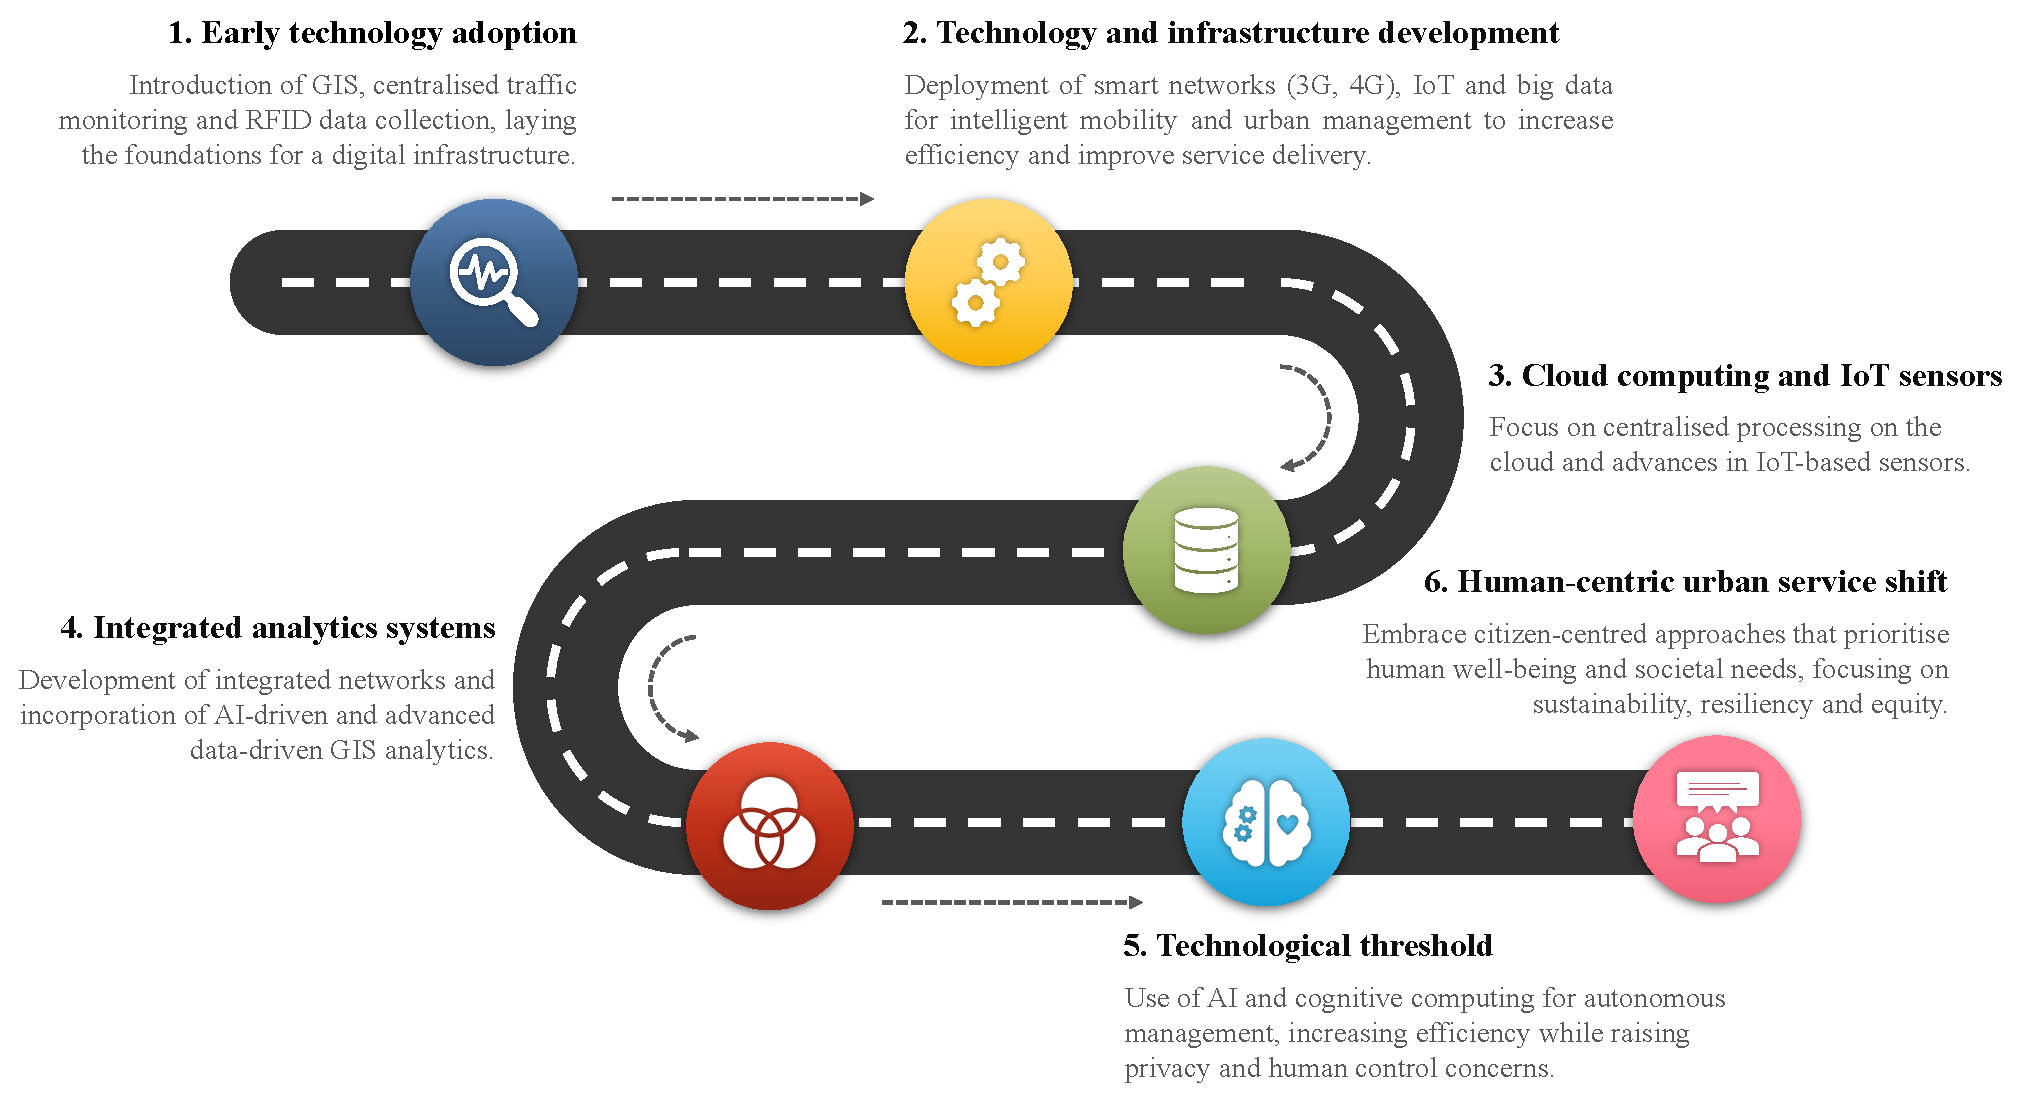
\includegraphics[width=0.9\linewidth]{figures/smart_city_roadmap.pdf}
    \end{adjustwidth}
    \caption{The evolutionary path of smart cities towards intelligent urban environments.}
    \label{fig:historical}
\end{figure}

The evolution of smart cities has not been straightforward, and there is considerable debate about classifying and organizing different stages of their development. However, some trends are particularly significant and deserve special attention, described as follows:

\begin{enumerate}
    %1
    \item Initially, the fundamental idea was to provide Geographic Information Systems (GIS)-based tools in conjunction with other solutions for centralized monitoring and data collection in urban environments \cite{costaAchievingSustainableSmart2024}. These technologies established the foundation for digital infrastructure, empowering city planners and managers to collect and analyze data related to urban environments in ways that were not previously feasible. While these advancements represented a significant step forward in urban management, they were primarily designed to serve administrative goals rather than directly improving the everyday experiences of citizens.

    %2
    \item As technology advanced, the focus of smart cities shifted towards more comprehensive data integration and infrastructure development. This period witnessed the implementation of sophisticated communication networks, including 3G and 4G wireless technologies, IoT-based systems, and advanced data analytics. These technologies facilitated a more interconnected environment in which systems could communicate and respond to one another in real time. The primary objective was to enhance efficiency and optimize service delivery across various urban domains.

    %3
    \item The third phase in the evolution of smart cities represents a fundamental transition towards a more participatory approach, characterized by an enhanced focus on community engagement and predictive capabilities. At this stage, crowdsourced solutions have emerged as a means of processing large amounts of data from sources like smartphones. The objective was to foster collaboration between the city and its residents, predicting urban trends and requirements. 

    %4
    \item Building on previous advances, the focus shifted towards integrated artificial intelligence and autonomous systems. This phase encompasses the advent of integrated networks and technologies, including autonomous vehicles, smart grids, and AI-driven resource management systems. In this phase, the objective was to deliver better (and sometimes sustainable) urban services capable of responding to immediate challenges and anticipating future needs, representing a step closer to the ideal of an intelligent city. 

    %5
    \item The more recent transformation in this urban development process can be observed in the advent of autonomous and cognitive cities, where AI and cognitive computing facilitate autonomous governance across urban basic functions. The smart city focus has been shifting towards human-centered design and the incorporation of privacy concerns, although such concerns are sometimes in their infancy in practical terms.
    
    %6
    \item The contemporary notion of a smart city has to be centered around urban environments that are effective and responsive to citizens' needs and behaviors. In fact, it is recognized that while technology can enhance urban life, it must be deployed in ways that respect and empower all citizens. Therefore, sustainability, equity, and resilience must be the fundamentals of the ultimate generation of smart cities, which will elevate the notion of intelligent cities to a more holistic and socially responsible one.
\end{enumerate}

As could be seen, there has been a persistent trend of creating ``smart'' environments by deploying cutting-edge technologies without fully understanding or addressing the unique and evolving needs of urban populations. While improving quality of life has consistently been a central goal, this objective is often approached from a superficial perspective. The definition of what makes a city smart is rather subjective, and there is a common misconception that ``smart'' automatically means ``better''. This conceptual misunderstanding has led to the allocation of public funds toward smart city initiatives that do not necessarily benefit the majority of citizens.

Despite the initial aspiration to elevate the quality of life, the advancement of smart cities has been mostly driven by the efficiency of public services. The initial phases of the smart cities road map were marked by technological determinism, where ``smartness'' was primarily defined by the sophistication of digital infrastructure. However, as cities have progressed through the aforementioned stages, there has been a growing recognition that technology alone cannot create truly intelligent cities. This rethinking will eventually lead to a shift towards a more participative and adaptive urban development and management paradigm, where the needs, preferences, and voices of citizens, along with environmental considerations, are central to an enhanced perception of quality of life.

We believe that the intelligent city paradigm will focus on creating environments that are not only technologically smart but also intelligent in their ability to foster well-being, safety, equity, and sustainability for all residents.


%%%%%%% 3.2
\subsection{The Intelligent Cities paradigm}
% Conceptual underpinnings of Intelligent Cities.
% [JOAO]
The smart city paradigm has evolved significantly since its inception, as previously mentioned. Nowadays, following several development phases, a gradual shift from a technology-centric focus to one that prioritizes human well-being and societal needs has already become apparent~\cite{singhDecadeReviewSmart2022,SCInclusiveFuture}. In fact, the current evolution trend of smart cities centers on advancing technologies to drive urban innovation in a sustainable, resilient, and equitable manner, although it remains a slow process. Recently, technologies such as AI-driven analytics, adaptive networks, and digital twins have provided advanced monitoring capabilities~\cite{zengSensorsInternetThings2024}, optimized network connectivity~\cite{resilienceSC1}, and various smart appliances~\cite{kumarEnergyEfficientSmartComfort2014,saeedIoTBasedIntelligentModeling2018,Singh2023}, enhancing overall efficiency within smart cities. This array of solutions primarily aims to improve the efficiency of urban services and promote environmental sustainability. However, the question of equitable availability and reliability of these advancements remains unresolved. 

%aqui ta lindo
Although the smart city model established the foundation for technological integration in urban environments, it frequently neglected the broader socioeconomic and cultural contexts that influence urban life~\cite{SCHappiness}. Consequently, the concept of intelligent cities emerged to build upon the technological foundations of smart cities by embedding these advancements within a comprehensive framework that prioritizes human well-being, equity, and resilience. In this sense, intelligent cities build on the foundation of smart cities by embedding advanced technologies within a comprehensive framework that integrates social and economic considerations. This concept ensures that cities prioritize not only technological advancements but also citizen-centered decision-making. This participatory approach would promote sustainable and equitable development by empowering citizens and integrating their needs into the urban planning process.

Building on this foundation, intelligent cities can enhance public services and safety while promoting inclusivity and ensuring that all citizens have access to quality healthcare and housing~\cite{SmartLivingDimension}. A commitment to sustainable resource management and ecological conservation helps cities stay resilient in the face of environmental challenges. Additionally, intelligent cities prioritize equitable transportation solutions to promote accessibility and improve mobility for all residents. Beyond technological innovation, economic development emphasizes job creation and economic inclusivity, ensuring that opportunities are available to diverse demographic groups~\cite{SCInclusiveFuture}. Education and lifelong learning are also central to intelligent cities, empowering citizens with the skills necessary for meaningful participation in a digital society. Lastly, intelligent cities are dedicated to ensuring transparency in public administration and fostering a participatory governance process.

%Achei top
By integrating these innovative dimensions into urban planning, intelligent cities will meet immediate societal needs and align with the United Nations' 2030 Sustainable Development Goals, extending beyond SDG 11 (Sustainable Cities and Communities). In fact, by fostering inclusive job markets and equitable employment opportunities, intelligent cities promote SDG 1 (No Poverty) and SDG 8 (Decent Work and Economic Growth). Moreover, incorporating technology into educational systems and enhancing digital literacy aligns with SDG 4 (Quality Education), ensuring all citizens have access to equitable lifelong learning opportunities. Smart cities also support SDG 6 (Clean Water and Sanitation) and SDG 7 (Affordable and Clean Energy) by utilizing smart technologies to optimize sustainable resource management and ensure fair distribution. Finally, by emphasizing energy efficiency and effective resource management, smart cities contribute to SDG 13 (Climate Action), reducing environmental impact and enhancing urban resilience.

As shown in Figure~\ref{fig:overview_of_intelligent_cities}, intelligent cities uphold their core principles of sustainability, resilience, and equity in a citizen-centered approach. This visual also illustrates the interplay between technological advancements and the smart city dimensions, emphasizing the strategic vision of intelligent cities to balance urban innovation with social goals.

\begin{figure}[htp]
    \centering
    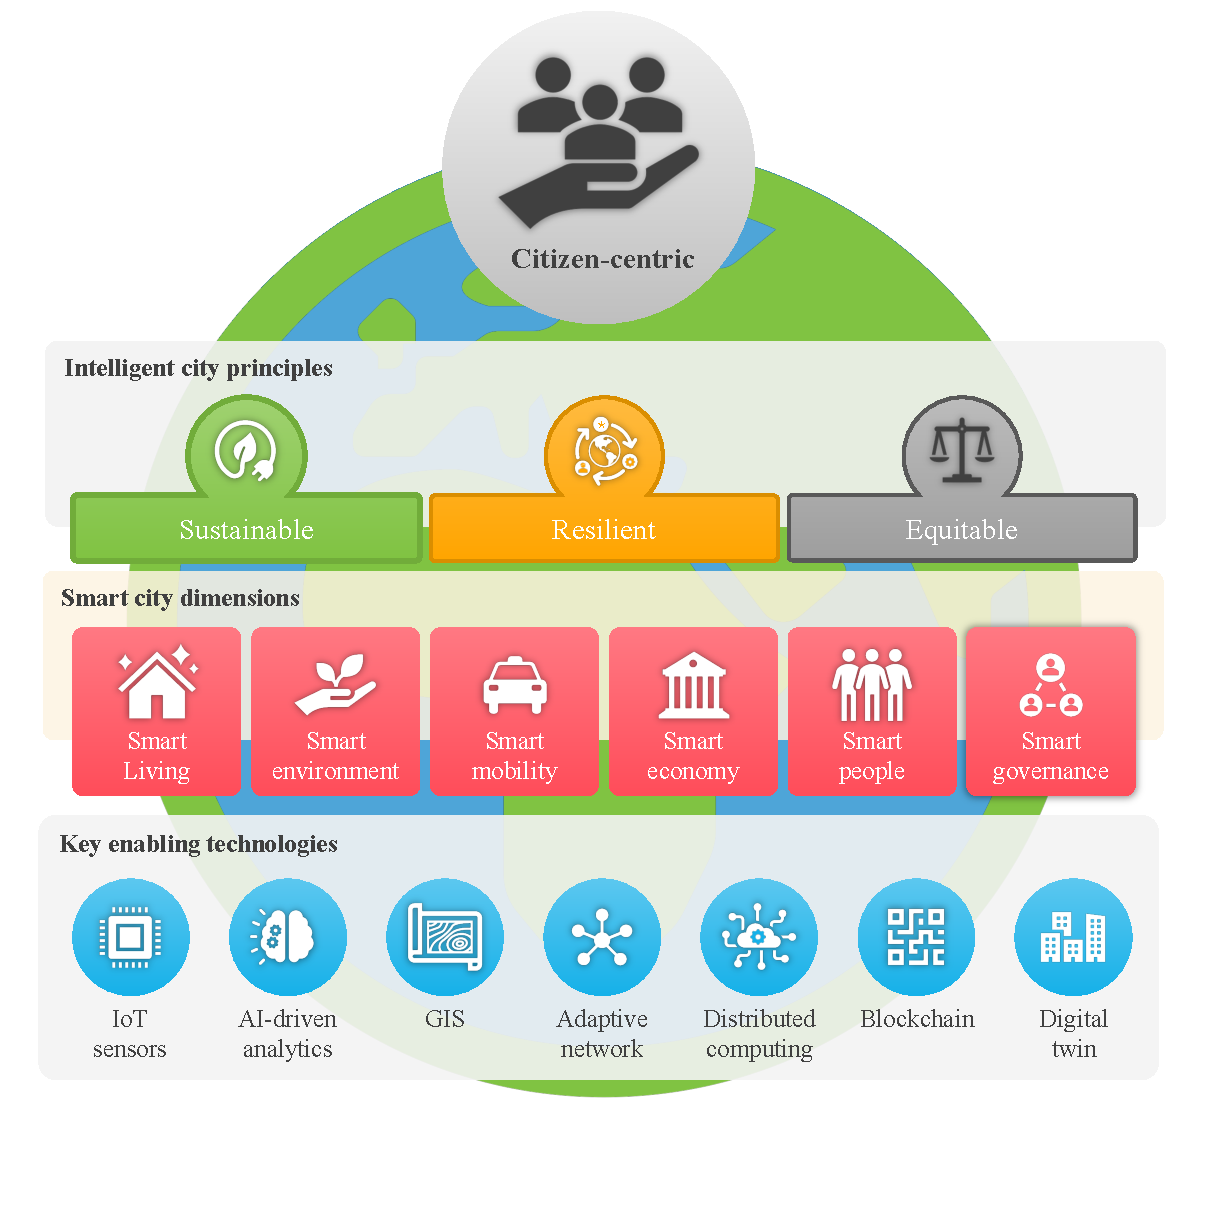
\includegraphics[width=0.75\linewidth]{figures/overview_intelligent_cities.pdf}
    \caption{Integration of intelligent city principles, focusing on the citizen-centered technological advancements within smart cities domains.}
    \label{fig:overview_of_intelligent_cities}
\end{figure}

This conceptual representation acknowledges that while technology plays a crucial role in maintaining and enhancing urban services, it must be utilized to meet the needs of all city residents. Therefore, technological advancements should tackle practical issues that directly impact smart city domains, encouraging a responsive and adaptive infrastructure that prioritizes elements affecting our daily lives. The goal is not merely to implement cutting-edge technology but to leverage it for balanced urban development, ensuring that the benefits of urbanization are felt by those whom the solutions are meant to address.

Although the rationale behind the concept of intelligent cities is not new~\cite{SCInclusiveFuture,SCHappiness,repetteCityAsPlatformDevelopment2021,ParticipatoryGovernanceNYC,bibriSustainableCitiesTechnologies2023}, integrating it with technology research and development, focusing on sustainability, resilience, and equity, remains a significant challenge. By incorporating the ``intelligent'' concept, cities can address current needs without compromising the ability of future generations to satisfy their own. This involves advancing technologies that reduce negative impacts and encourage efficient, future-oriented resource management.

The interrelationship between sustainability, resilience, and equity within the urban technology domain is critical for the successful development of cities and must be addressed holistically. A sustainable city that lacks resilience may struggle to cope with environmental change, undermining its sustainability goals. Conversely, a city that prioritizes technological advancement without concurrently implementing equitable resource distribution and inclusive policies increases the risk of exacerbating existing social inequalities. Indeed, if access to the benefits of innovation is confined to privileged groups, the socioeconomic divide will widen further. Therefore, to provide a comprehensive understanding of the benefits of intelligent cities and how technology can be utilized to achieve them, this paper supports the view that intelligent cities must encompass two domains:

\begin{itemize}
    \item \textbf{Social domain:} Integrating social factors into urban development improves accessibility, promotes equity, and encourages community engagement. As a result, intelligent cities embrace a human-centric design approach to make sure that technological advancements contribute to increasing the livability and inclusivity of urban environments. This involves creating opportunities for citizens and ensuring access to essential services so that cities can effectively fulfill their fundamental functions.

    \item \textbf{Technology domain:} The development of intelligent cities relies on creating digital infrastructures to collect and analyze data that anticipates trends and automates processes in a predictive and adaptive way. These technological foundations provide the frameworks for making well-informed decisions and achieving efficient resource management.
\end{itemize}

It is important to recognize that these domains are interdependent, each supporting and enhancing the others. The intersection of the inherent elements differentiates an ``intelligent'' city from a ``smart'' city. In intelligent cities, technology serves not as an end but as a means to achieve broader societal goals. This sociotechnical approach ensures that the benefits of urban innovation are widely shared and contribute to urban health and prosperity. The following subsections examine how these domains relate to sustainability, resilience, and equity in practical urban functions, exploring current solutions and challenges in integrating these principles.

\subsection{Urban social domain}
% [JOAO]
The urban social domain encompasses the collective social interactions and functions within urban environments. It includes various aspects of daily life, such as housing, employment, education, healthcare, and recreational activities~\cite{carlosmoreno15}. Each of these functions plays a distinct but integrated role in shaping the overall urban experience and contributing to the well-being of residents. Together, these functions form a crucial element of urban life, illustrated as follows. 

\begin{enumerate}
    \item \textit{Living:} Housing is a fundamental part of urban life, and the availability of affordable, quality housing is crucial for social stability. Intelligent cities need to prioritize inclusive housing policies that accommodate diverse populations and promote social equity. Moreover, citizens should have equal access to the benefits of smart services and home appliances.

    \item \textit{Working:} Employment opportunities are crucial for economic sustainability. Intelligent cities can leverage the advantages of smart systems to create effective job opportunities, enhance workforce development, and support local businesses. Nevertheless, it is important to ensure these opportunities are accessible to all residents, regardless of their socioeconomic background.

    \item \textit{Supplying:} The supply of goods and services is essential to urban life. Smart logistics and supply chain management can improve the efficiency of urban economies. This also encompasses sustainable energy and water supply, along with effective waste collection. However, it is important to consider the social implications of these systems, such as access to essential services for marginalized communities.

    \item \textit{Learning:} Education is a key component of the urban social domain. Intelligent cities can leverage technology to improve educational opportunities, encourage innovative learning methods, and ensure that all residents have access to quality education. This is particularly important for tackling social inequalities and promoting community engagement. 

    \item \textit{Caring:} Healthcare and safety services are crucial for the well-being of urban populations. Intelligent cities must prioritize equitable access to healthcare services, using technology to enhance health outcomes and address disparities in healthcare availability. Additionally, they must concentrate on preventive measures to reduce crime and bolster emergency resilience.

    \item \textit{Enjoying:} Recreational and cultural activities enhance the quality of life in urban environments. Thus, intelligent cities should support inclusive public spaces and cultural initiatives that encourage community engagement and social cohesion.
\end{enumerate}

These basic social functions form the main reason for the growing appeal of city life and the increasing urban population. These functions represent the essential aspects of daily life that cities are uniquely equipped to provide on a large scale and with variety~\cite{SCDimensions}. Urban environments offer a wealth of opportunities and resources that cater to diverse needs and lifestyles, ranging from varied housing options and dynamic job markets to accessible education and healthcare services~\cite{SCQualityOfLife}. The promise of richer cultural and recreational activities also draws people to urban areas, offering a more engaging quality of life~\cite{SCHappiness}. The dense network of these social functions creates an ecosystem that fosters economic opportunity and social interaction, attracting individuals in search of better prospects and improved living conditions.

The concept of intelligent cities encompasses multiple smart dimensions, as illustrated in Figure~\ref{fig:overview_of_intelligent_cities}. These dimensions are interrelated and collectively contribute to the effectiveness of urban functions. Investments in human and social capital, along with advancements in urban infrastructure and governance policies, are essential for achieving greater social and economic efficiency \cite{TopDownGov1}. This interconnectedness underscores the importance of a comprehensive approach to urban planning, where each dimension supports and enhances the others.  

The following subsections further discuss how the aforementioned social functions are inherently associated with the development of intelligent cities. 

\subsubsection{Citizen engagement and governance}

One of the primary social improvements associated with modern cities is strengthening citizen engagement and participation in governance processes. In this context, intelligent cities provide platforms to facilitate citizen involvement in decision-making, fostering a sense of community and belonging~\cite{GenderEquitySC}. This participatory governance model ensures that urban policies reflect the diverse needs and aspirations of the population. The widespread integration of citizen feedback into urban planning processes leads to more responsive and adaptive governance, ultimately enhancing the living and enjoying urban function~\cite{CitizenParticipation}.  

The collaborative nature of intelligent cities—where various stakeholders, including government, the private sector, academia, and civil society, work together to achieve common goals—is another critical factor. This multi-stakeholder approach fosters innovation and ensures that diverse perspectives are considered in developing urban policies and initiatives~\cite{GenderEquitySC}. Governance models significantly shape urban policy implementation and can take different forms. Top-down governance centralizes decision-making at higher government levels, which can enable rapid policy action, as seen in Wuhan during the COVID-19 pandemic when strict lockdowns were swiftly enforced~\cite{TopDownGov1}. However, this model may lack community engagement and often fails to address specific local needs~\cite{GenderEquitySC}. In contrast, bottom-up governance prioritizes local participation, as demonstrated by Porto Alegre's participatory budgeting, which enhances civic engagement by allowing citizens to influence local budgets~\cite{ParticipatoryBudgeting}. However, this model can encounter resource constraints and coordination challenges in larger cities. 

Intelligent cities strive for a hybrid governance model that balances top-down authority with bottom-up participation, integrating citizen input while maintaining centralized oversight. For example, Copenhagen employs this model to reconcile sustainability initiatives with community feedback 
\cite{CitizenParticipation, SCStakeholders}. This approach enables the successful execution of sustainability initiatives, such as climate action plans, by incorporating community feedback while ensuring alignment with broader governmental objectives. Therefore, by creating an ecosystem of collaboration, intelligent cities can utilize the strengths of various sectors to tackle complex urban challenges more effectively. 

\subsubsection{Inclusivity and accessibility}

Intelligent cities prioritize inclusivity and accessibility, ensuring that all residents, regardless of socioeconomic status, can benefit from urban innovations. Initiatives aimed at enhancing public transportation systems through smart mobility solutions can significantly improve access to essential services, such as healthcare and education, particularly for marginalized communities 
\cite{SCStakeholders}. By addressing social inequities, intelligent cities contribute to a more equitable urban environment where all citizens can thrive. An example of a successful implementation of a social equity strategy is Barcelona's ``Superblocks'' initiative 
\cite{BarcelonaSuperblocks}. While reducing traffic and creating pedestrian-friendly spaces, this project also focuses on integrating green areas within these superblocks, making urban areas more inclusive for all residents.

Medellín has transformed its urban landscape through inclusive policies aimed at reducing socioeconomic disparities. The city implemented the ``Metrocable'' system, a cable car that connects low-income neighborhoods to the city center, facilitating access to jobs and services \citet{MetroCable}. Recognizing the importance of equitable access to green spaces and urban forestry, Accra has initiated programs to enhance tree cover, addressing environmental inequalities that disproportionately affect these communities \cite{AccraGreenSpaces}. By involving residents in tree planting and maintenance, the city enhances urban biodiversity and fosters community ownership and pride. 

\subsubsection{Environment and green cities}

The environmental aspect of intelligent cities is equally essential, as it includes strategies to promote sustainability and resilience in urban ecosystems while improving the quality of life. Environment-centered solutions, such as those that support waste management systems, energy-efficient infrastructure, and efficient water distribution practices, are crucial in minimizing the ecological footprint of cities \cite{IntegraedCity}. While advancing the sustainability of urban environments, these technologies also contribute to better public health outcomes by decreasing pollution and encouraging cleaner air and water.

Furthermore, incorporating green spaces and sustainable urban design principles within intelligent cities promotes a healthier living environment. In fact, access to green spaces is associated with improved mental health and well-being, as well as increased social interactions among residents 
\cite{GreenSpaces}. By prioritizing the development of parks, community gardens, and recreational areas, intelligent cities enhance their inhabitants' overall quality of life, encouraging physical activity and social cohesion. The Singapore Green Plan 2030 is a successful example of fostering sustainability and resilience in the city-state. It includes various initiatives that provide significant benefits across multiple dimensions, including environmental, social, and economic 
\cite{SingaporeGreenPlan}. The focus on sustainable urban design and green buildings improves the quality of living spaces, making them more suitable for healthy lifestyles.

The waste management strategy developed by Yokohama is a notable example of how intelligent cities can promote environmental sustainability. The city has implemented a comprehensive waste management plan that emphasizes waste reduction, recycling, and public involvement. This strategy has established a strong recycling program, achieving a recycling rate of over 30\% for municipal solid waste~\cite{WasteManagement1}. Enhancements in waste collection services can optimize collection routes and decrease landfill waste. Moreover, Amsterdam is recognized for its integrated approach to urban water management~\cite{WaterManagement1}. The city employs a comprehensive framework known as the ``Blue City Index'', which evaluates its water management practices across various indicators, including water quality, availability, and infrastructure efficiency. Finally, there has been a remarkable transition to more sustainable energy sources in the past two decades~\cite{SustainableEnegy1,SustainableEnergy2}. These developments exemplify how sustainable energy systems can improve efficiency and resilience.

\subsubsection{Economic development}

Intelligent cities are also expected to foster economic development through innovation and entrepreneurship. Establishing supportive ecosystems for startups and small businesses, especially those led by women and historically marginalized groups, is essential for driving economic growth~\cite{SupportiveEcossystem}. By providing access to resources, mentorship, and networking opportunities, smart cities not only stimulate local economies but also create job opportunities, thereby enhancing the overall well-being of their residents. The ``StartupAmsterdam'' initiative serves as a prime example, focusing on developing a startup ecosystem that supports diverse entrepreneurs~\cite{StartupAmsterdam}. The program provides mentorship, access to funding, and networking opportunities, particularly for women and minority entrepreneurs. 

The development of intelligent cities has the potential to transform the social aspects of urban functionality within the context of smart urban living. This can be achieved through a comprehensive and integrated approach to planning these urban spaces. By fostering citizen engagement, promoting inclusivity, and prioritizing sustainability, it has been shown that cities can create urban environments that enhance the quality of life for all residents. This ongoing evolution will continue to shape the future of urban living, addressing the pressing challenges of our time while promoting resilience and well-being. 

\subsection{Urban technology domain}
%[THIAGO]
Transforming smart cities into intelligent cities involves a comprehensive rethinking of how urban technologies are employed to support the diverse and evolving needs of residents. While previous phases of smart cities have emphasized enhancing efficiency and optimizing urban functions through technology, intelligent cities will take a more integrated and holistic approach that blends technological advancements with human-centric values and principles. This shift is crucial for addressing the complex challenges facing urban areas, from environmental sustainability to social equity and resilience against disruptions~\cite{kirimtatFutureTrendsCurrent2020,Trindade2017,singhDecadeReviewSmart2022}. Therefore, to achieve these goals, technologies deployed in intelligent cities must be innovative but also sustainable, resilient, and equitable.

%3.4.1
\subsubsection{Technological landscape}

Sustainability, resilience, and equity serve as the foundational principles for deploying technology in intelligent cities. First, sustainable technologies are those that minimize environmental impacts, optimize resource usage, and foster circular economies~\cite{Hu2018,SustainableEnegy1}. These technologies contribute to reducing carbon footprints, conserving energy, and enhancing overall resource management by ensuring urban systems operate efficiently and responsibly. For instance, IoT sensors embedded throughout the city can monitor air quality, energy consumption, and waste production in real-time, allowing for immediate adjustments to reduce emissions and resource use~\cite{zengSensorsInternetThings2024,SensorsSustainable2021}. Resilient technologies, in contrast, are designed to adapt to and recover from various disruptions, such as natural disasters, cyberattacks, or infrastructural breakdowns~\cite{resilienceSC1,ReliabilityDetectability_CCF_EMS}. These technologies integrate built-in redundancies, flexibility, and adaptability to ensure continuous operation and quick failure recovery. Finally, equitable technologies are geared towards ensuring all citizens have fair access to urban services, regardless of socioeconomic status, age, gender, or ability. They avoid reinforcing existing inequalities by promoting inclusivity and accessibility, such as AI-driven platforms that provide personalized public services to cater to diverse needs~\cite{ButtazzoniEquitySC}.

The transition from smart to intelligent cities thus involves the strategic use of various core technologies, including IoT sensors, AI-driven analytics, Geographic Information Systems, adaptive networks, distributed computing, blockchain, and digital twins~\cite{kirimtatFutureTrendsCurrent2020} (see Figure~\ref{fig:overview_of_intelligent_cities}). These technologies, either individually or in combination, as depicted in Figure~\ref{fig:Technologies}, can significantly enhance different dimensions of urban life (such as smart living, smart environment, smart mobility, smart economy, smart people, and smart governance) to create cities that are efficient, sustainable, resilient, and equitable.

\begin{figure}[htb]
    \centering
    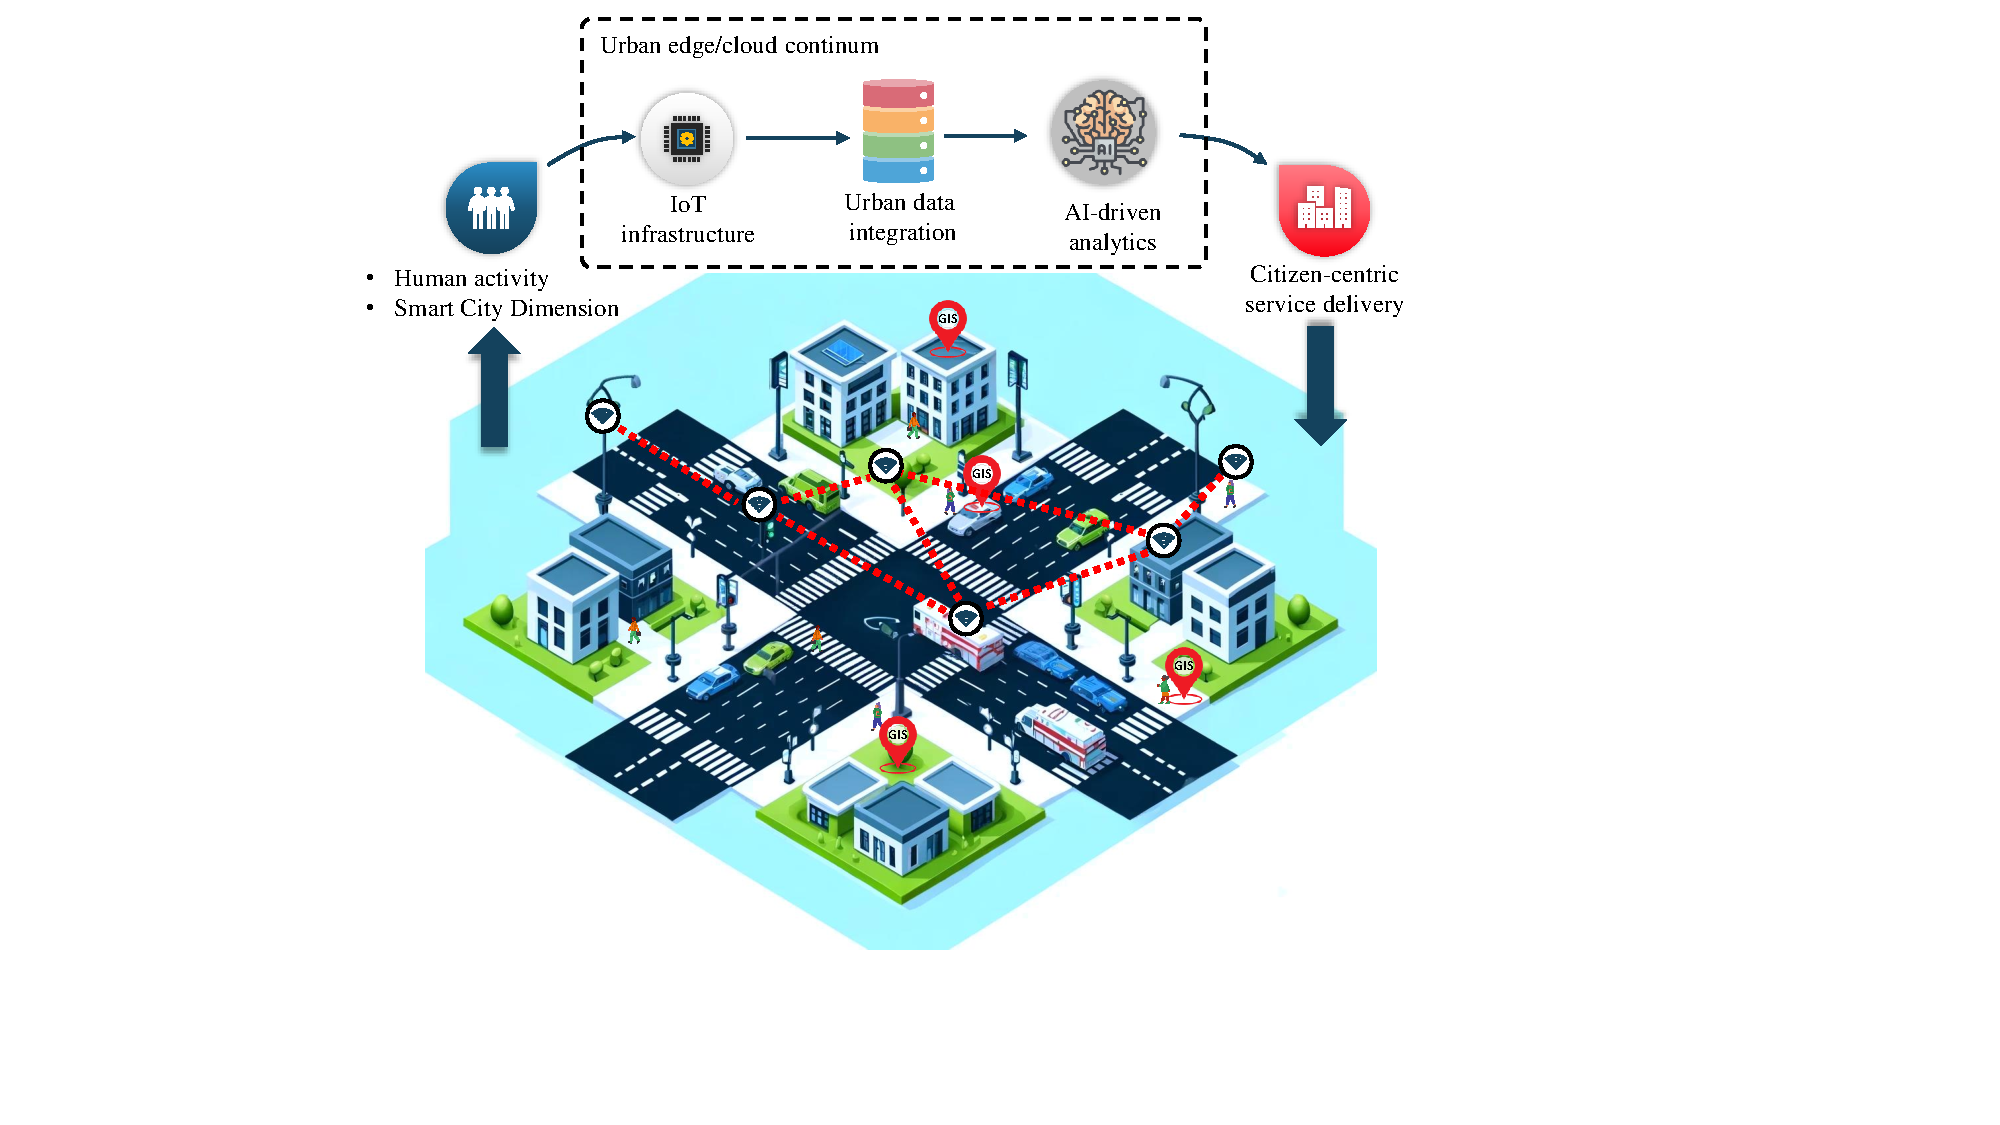
\includegraphics[width=0.85\linewidth]{figures/Technologies_v2.pdf}
    \caption{Technologies integration to foster citizen-centric intelligent cities.}
    \label{fig:Technologies}
\end{figure}

IoT sensors are fundamental to gathering real-time data across various urban domains, including traffic management, energy consumption, water usage, and environmental quality. By integrating this data with AI-driven analytics, cities can generate actionable insights and automate decision-making processes that optimize resource allocation and service delivery~\cite{costaSurveyEmergenciesManagement2022, duSensableCitySurvey2019}. For example, AI can personalize healthcare and educational services, providing targeted interventions and optimizing resource use to enhance urban living standards~\cite{PachecoRocha2019}. GIS add another layer of spatial analysis, offering critical insights for urban planning and management. When integrated with IoT and AI, GIS help cities map out green spaces, flood zones, and pollution hotspots, facilitating sustainable urban growth while ensuring equitable access to resources and services~\cite{costaAchievingSustainableSmart2024}.

The integration of adaptive networks and distributed computing significantly enhances the functionality of intelligent cities by enabling more responsive and flexible management of urban systems~\cite{javedFutureSmartCities2022}. These technologies facilitate dynamic load balancing and ensure continuous service delivery, even during peak demand or system failures. For example, adaptive networks in intelligent cities can dynamically manage electricity distribution by balancing supply and demand in real-time, thereby optimizing energy use~\cite{EnergyReconfigurableDistributionNetworks}. Distributed computing, particularly when supported by the concept of cloud-edge continuum, enables seamless data processing both centrally in the cloud and at the network's edge. This setup allows for swift, localized decision-making in critical real-time applications, such as emergency healthcare and traffic management, while still leveraging the extensive computational power of cloud resources for more complex analyses~\cite{EdgeCloudContinuum}. This system architecture also supports connected vehicles and smart traffic management systems, providing real-time updates that improve road safety and reduce congestion~\cite{barodiIntelligentTransportationSystem2023}.

Digital twins, as virtual replicas of physical urban environments, provide an innovative approach to enhancing urban planning. By allowing cities to simulate a variety of scenarios, digital twins enable urban planners to optimize the use of resources and design more sustainable cities. These simulations help anticipate potential risks, such as natural disasters, climate change impacts, or infrastructure failures, and test interventions without putting residents in harm's way, thereby bolstering urban resilience~\cite{UrbanDigitalTwinChallenges,DigitalTwinDisaster}. The ability to forecast and respond to such challenges before they occur ensures that cities can maintain functionality and service delivery even under adverse conditions. Furthermore, digital twins enable more proactive and informed data-driven decision-making processes by providing a dynamic tool for visualizing the impact of policy decisions~\cite{DigitalTwinsSurvey,TrendsDigitalTwinFrameworkArchitectures}.

Therefore, by supporting sustainability through resource efficiency, resilience through real-time monitoring and adaptability, and equity through inclusive access to services and opportunities, the core technological pillars of intelligent cities would help to create urban environments that are better equipped to meet the challenges of the citizen-centric future.

%3.4.2
\subsubsection{Challenges and technical issues}

Similarly to the smart cities context, but on a larger scale, building intelligent cities presents several challenges yielded by the deployment of such integrated and informed technology systems in urban settings. Some of the main issues are related to privacy, security, trust, digital equality, and the avoidance of bias~\cite{BridgingEthicsPractice,EthicsSmartCityAI}. Intelligent cities solutions naturally collect and process vast amounts of personal data, raising significant privacy and security concerns. Without robust safeguards, smart city infrastructure could expose sensitive information, making it vulnerable to cyberattacks and data breaches. To address these risks, cities must implement strong cybersecurity measures, data encryption protocols, and adopt privacy-by-design principles. The failed ``Sidewalk Labs'' project in Toronto illustrates the importance of having clear data governance frameworks that define how data is collected, used, stored, and shared to protect residents' privacy~\cite{SidewalkToronto_Trust}.

Trust is another critical factor in the success of intelligent cities~\cite{TrustworthyAIReview}. The use of opaque AI algorithms in urban decision-making systems, such as traffic management and public safety, can lead to biased outcomes, prioritizing traffic flow in wealthier regions over less affluent areas or identifying minority neighborhoods as high-risk areas, which undermines public trust. To foster trust, cities need to adopt transparent AI frameworks, such as Amsterdam's and Helsinki's AI registers~\cite{AmsterdamHelsinki_1}, which provide residents with information about AI usage and decision-making processes. Participatory governance models, such as Boston's ``Smart City Playbook''~\cite{BostonSmartCityPlaybook}, also help build trust by involving citizens in the design and decision-making processes, ensuring that technology deployment aligns with community values.

Digital equality poses a significant challenge, as the deployment of advanced technologies could widen the digital divide if not all residents have equal access to digital tools and internet connectivity. Marginalized groups, such as low-income communities and the elderly, are particularly vulnerable to being excluded from smart city benefits. To promote digital equality, cities must ensure equitable access to digital infrastructure and resources through inclusive policies. The ``Barcelona Digital City'' plan~\cite{BarcelonaDigitalCity}, for example, promotes public digital infrastructure and digital literacy programs to ensure all citizens can benefit from intelligent city advancements.

Avoiding bias in AI-driven decision-making processes is crucial to prevent reinforcing social inequalities. Biased algorithms in areas such as facial recognition and predictive policing can lead to discriminatory outcomes. To mitigate these risks, cities should adopt ethical AI guidelines that require regular algorithmic audits and involve diverse stakeholders in AI development~\cite{EthicsSmartCityAI}. Policy frameworks are evidenced by the European Union's ``Ethics Guidelines for Trustworthy AI''~\cite{TrustworthyAIReview} and New York City's ``Automated Decision Systems Task Force''~\cite{ParticipatoryGovernanceNYC} provide models for ensuring fairness, transparency, and accountability in AI use. By adopting comprehensive policy frameworks and city-level initiatives, intelligent cities can safeguard residents' rights and promote ethical technology use, ensuring that technological advancements lead to inclusive, equitable, and sustainable urban environments.

Blockchain technology further contributes to addressing these trustworthy challenges in the development of intelligent cities. Blockchain, by design, enhances the security, transparency, and decentralization of data management, which is crucial for fostering trust and accountability in urban governance. Its immutable ledger can secure data used for decision-making processes, ensuring it remains transparent and tamper-proof~\cite{TechnologiesSolutionsSecurity,BlockchainSustainability}. This feature is especially beneficial for e-governance platforms, where blockchain can support transparent voting systems, public fund management, and secure data sharing among stakeholders without compromising residents' privacy. By ensuring that governance processes are auditable and transparent, blockchain builds public trust in digital governance systems and economic transactions, promoting a more inclusive and equitable governance framework. 

Therefore, by implementing robust ethical guidelines, participatory governance models, and transparent data management practices, intelligent cities can create environments where technological innovation directly supports the well-being and rights of all citizens, ensuring that urban development is both advanced and humane.


%%%%%%%%%%%%%%%%%%%%%%%%%%%%%%%%%%%%%%%%%%

\section{Evaluating intelligent cities worldwide}
\label{sec:comp}
% [JOAO, JUST]
%%% FONTES
% Barcelona: https://opendata-ajuntament.barcelona.cat/data/en/dataset
% Helsinki: https://hri.fi/data/en_GB/dataset
% Helsinki pontos de recarga: https://kartta.hel.fi/?setlanguage=en#
% São Paulo: http://dados.prefeitura.sp.gov.br/pt_PT/
% Buenos Aires: https://data.buenosaires.gob.ar/dataset/
% Buenos Aires pontos de recarga: https://www.plugshare.com/br

Many smart city initiatives have used technology to improve the quality of public services in urban areas. Additionally, numerous researchers are exploring novel technologies, methodologies, and conceptual frameworks aimed at enhancing urban living through these initiatives. Despite the growth of smart city applications, not all of them are as people-focused as they should be. One reason for this issue is the marketing use of the term ``smart city,'' which governments use to create the perception that smart cities are inherently superior. As discussed throughout this article, the idea of being smart is not necessarily linked to sustainability, equity, and resilience. Therefore, a new rationale for smart cities is necessary.  

To demonstrate that current smart cities are far from the concept of intelligent cities, three selected smart cities from various geopolitical contexts have been assessed based on their alignment with the principles of sustainability, equity, and resilience. Therefore, the following cities were chosen for analysis:

\begin{itemize}
    \item \textbf{Helsinki, Finland:} Recognized as one of the top 20 smart cities in the IMD Smart Cities Index 2024~\cite{imd2024}, Helsinki boasts a long history of smart city development. This city was chosen as a case study because it illustrates the unequal distribution of smart urban services, even in a city with a high Human Development Index (HDI).

    \item \textbf{Barcelona, Spain:} As a prime example of open data accessibility, the city of Barcelona has launched a ``New Data Deal'' program~\cite{barcelona_data_deal}, making its data publicly available through a web portal. This data includes various aspects of the city, comprising 571 datasets. The release of this data is a key component of the ``Barcelona Ciutat Digital'' strategy, which represents an important initiative in the realm of intelligent cities.
    
    \item \textbf{Buenos Aires, Argentina:} To illustrate how a metropolis in a developing country seeks to improve the quality of life for its residents, we have chosen Buenos Aires, which currently ranks 123rd in the IMD Smart Cities Index 2024. Our goal is to determine how a city in a developing nation that has adopted smart city strategies compares to those in developed regions in terms of intelligent city principles.

\end{itemize}

To evaluate the inconsistencies of smart city services related to sustainability, we examined the availability of Electric Vehicle (EV) charging stations and bike-sharing stations, as these are common smart city services~\cite{bittencourtSurveyAdaptiveSmart2024}. The shift from Internal Combustion Engine (ICE) vehicles to EVs can enhance air quality in urban areas by reducing $\text{CO}_2$ emissions, thus improving the livability of these environments~\cite{ev_qualidade_ar}. Similar benefits arise when bike sharing is promoted among citizens~\cite{bike_qualidade_ar}. While these two smart city initiatives cannot stop the greenhouse effect, they do significantly improve the quality of life for those living in large, dense urban centers.

Secondly, to determine the resilience of urban areas, a risk assessment of the urban zones was conducted using the ``CityZones'' tool~\cite{cityzones_flood}. This tool allows for the classification of zones within a defined area based on their resilience during an emergency. As a result, low-resilience zones are those that will need a longer recovery period after a disaster, whether due to a lack of response centers or their proximity to threats. In any case, implementing safety solutions is a priority to enhance urban resilience and ensure the safety of cities. In this context, our risk assessment will analyze the behavior of various city areas regarding resilience.

To evaluate the equity of the selected cities, open data sources were used to categorize neighborhoods based on the socioeconomic status of their residents. This classification aims to ensure that smart city solutions are accessible to everyone. Ideally, every citizen, no matter their social class, should benefit from the smart city initiatives implemented in the city. By incorporating these assessments, we can evaluate the inclusivity and effectiveness of these smart city solutions.

To gather all the necessary data for this evaluation phase, we utilized online open data sources. For Helsinki, we accessed ``Helsinki Region Infoshare''~\cite{dados_helsinki}, a government-supported data platform that provides official information from Helsinki, Espoo, Vantaa, and Kaunianen. For data on EV charging points, we chose the ``Helsinki Map Service''~\cite{dados_helsinki_ev}, offered by the city of Helsinki, which presents maps covering various topics. In Barcelona, we employed ``Open Data BCN''~\cite{dados_barcelona}. For Buenos Aires, we referred to ``Buenos Aires Data''~\cite{dados_buenos_aires}, released by the government of Buenos Aires, containing data in multiple formats. To check EV charging points, we relied on the ``PlugShare'' platform~\cite{dados_buenos_aires_ev}, an online service that shows the locations of EV charging stations worldwide.

Figures~\ref{fig:data_helsinki}, \ref{fig:data_barcelona}, and \ref{fig:data_buenos_aires} illustrate the sustainability and equity data for the three cities. Each neighborhood is color-coded based on citizens' socioeconomic status, where red represents the least wealthy areas and blue indicates the most wealthy. For the city of Barcelona (Figure~\ref{fig:data_barcelona}), the annual income per person has been analyzed using data provided by Open Data BCN. In contrast, the value of the square meter for Helsinki (Figure~\ref{fig:data_helsinki}) and Buenos Aires (Figure~\ref{fig:data_buenos_aires}) has been evaluated based on their respective open datasets. Both parameters serve as effective indicators of citizens' financial power. The maps reveal that the three cities display a concentration of both high- and low-income zones.

\begin{figure}[htb]
    \centering
    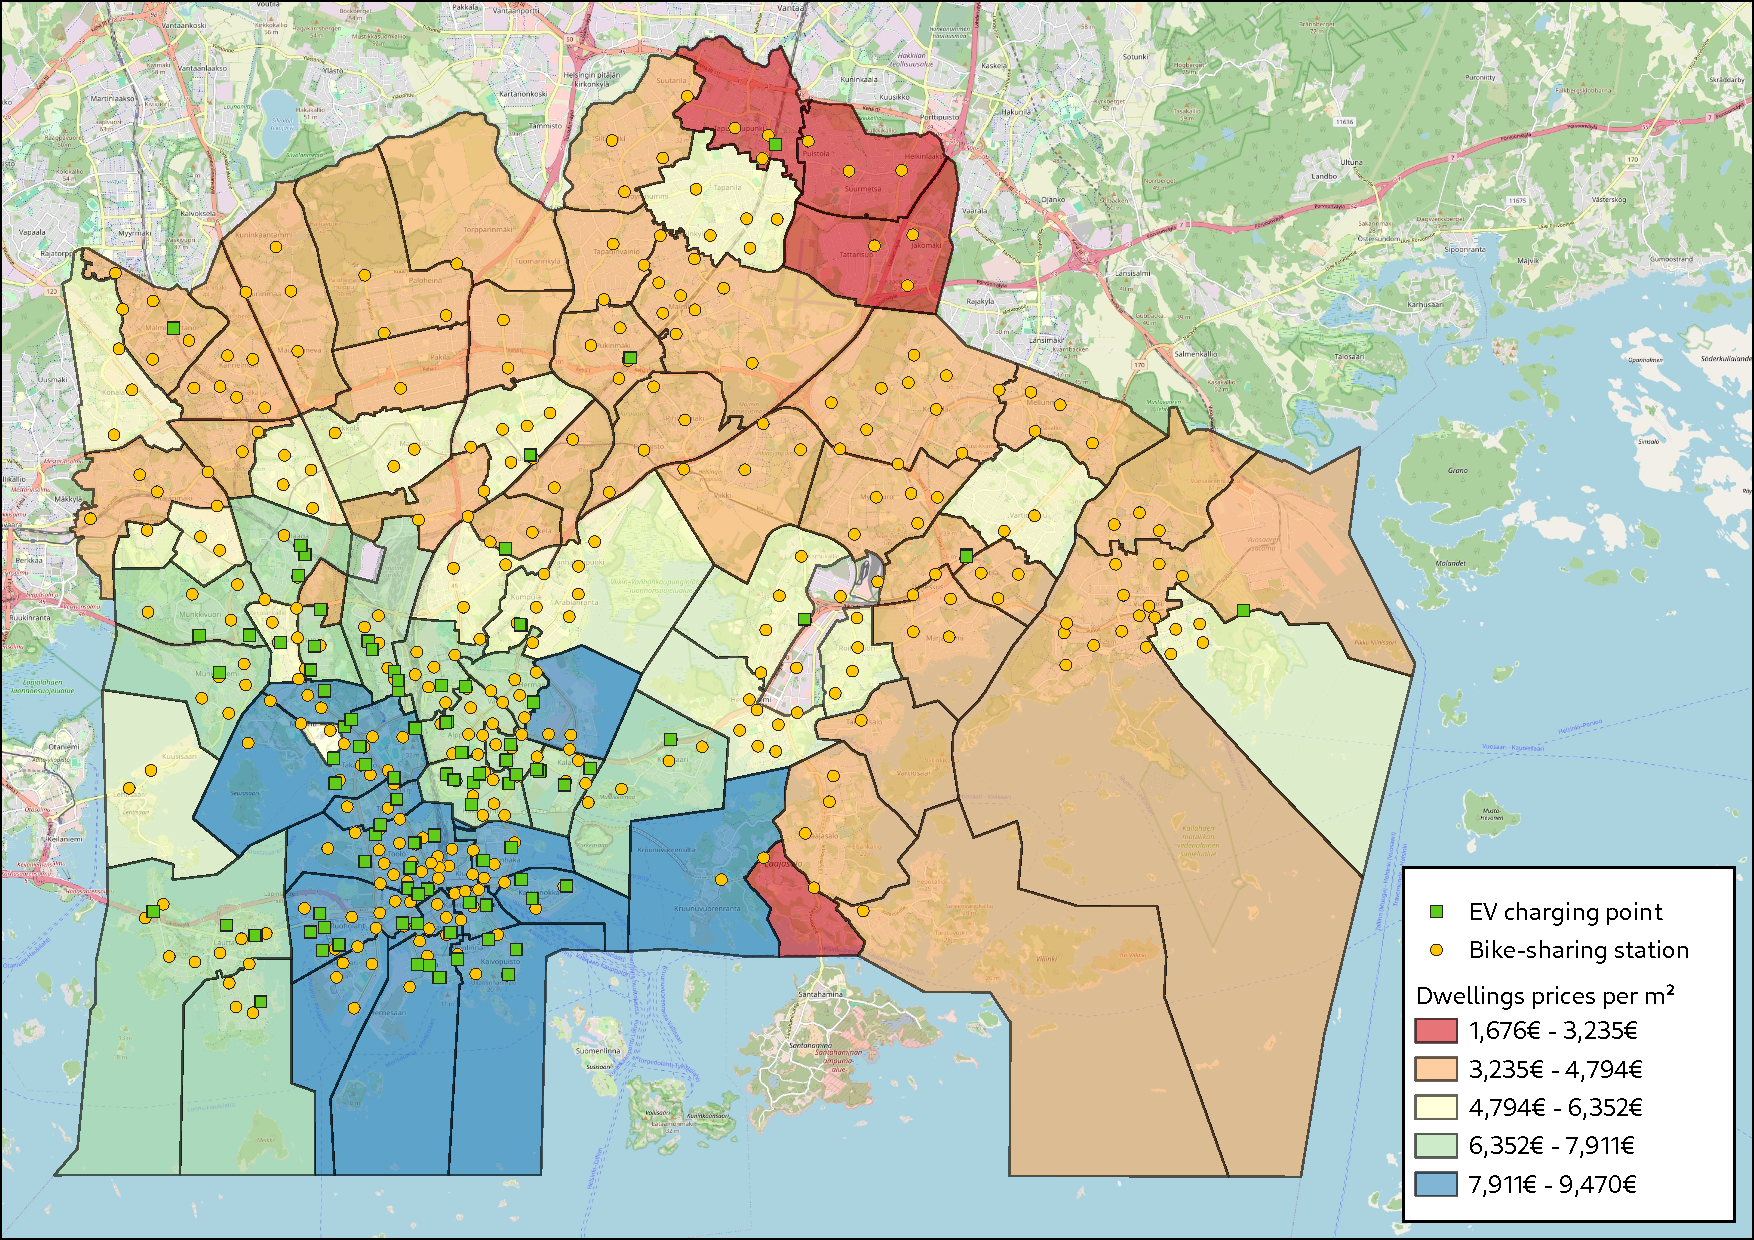
\includegraphics[width=\textwidth]{figures/Helsinki_data.pdf}
    \caption{Assessment of sustainability and equitable distribution of services in Helsinki, focusing on the placement of bike-sharing and electric vehicle charging stations.}
    \label{fig:data_helsinki}
\end{figure}

\begin{figure}[htb]
    \centering
    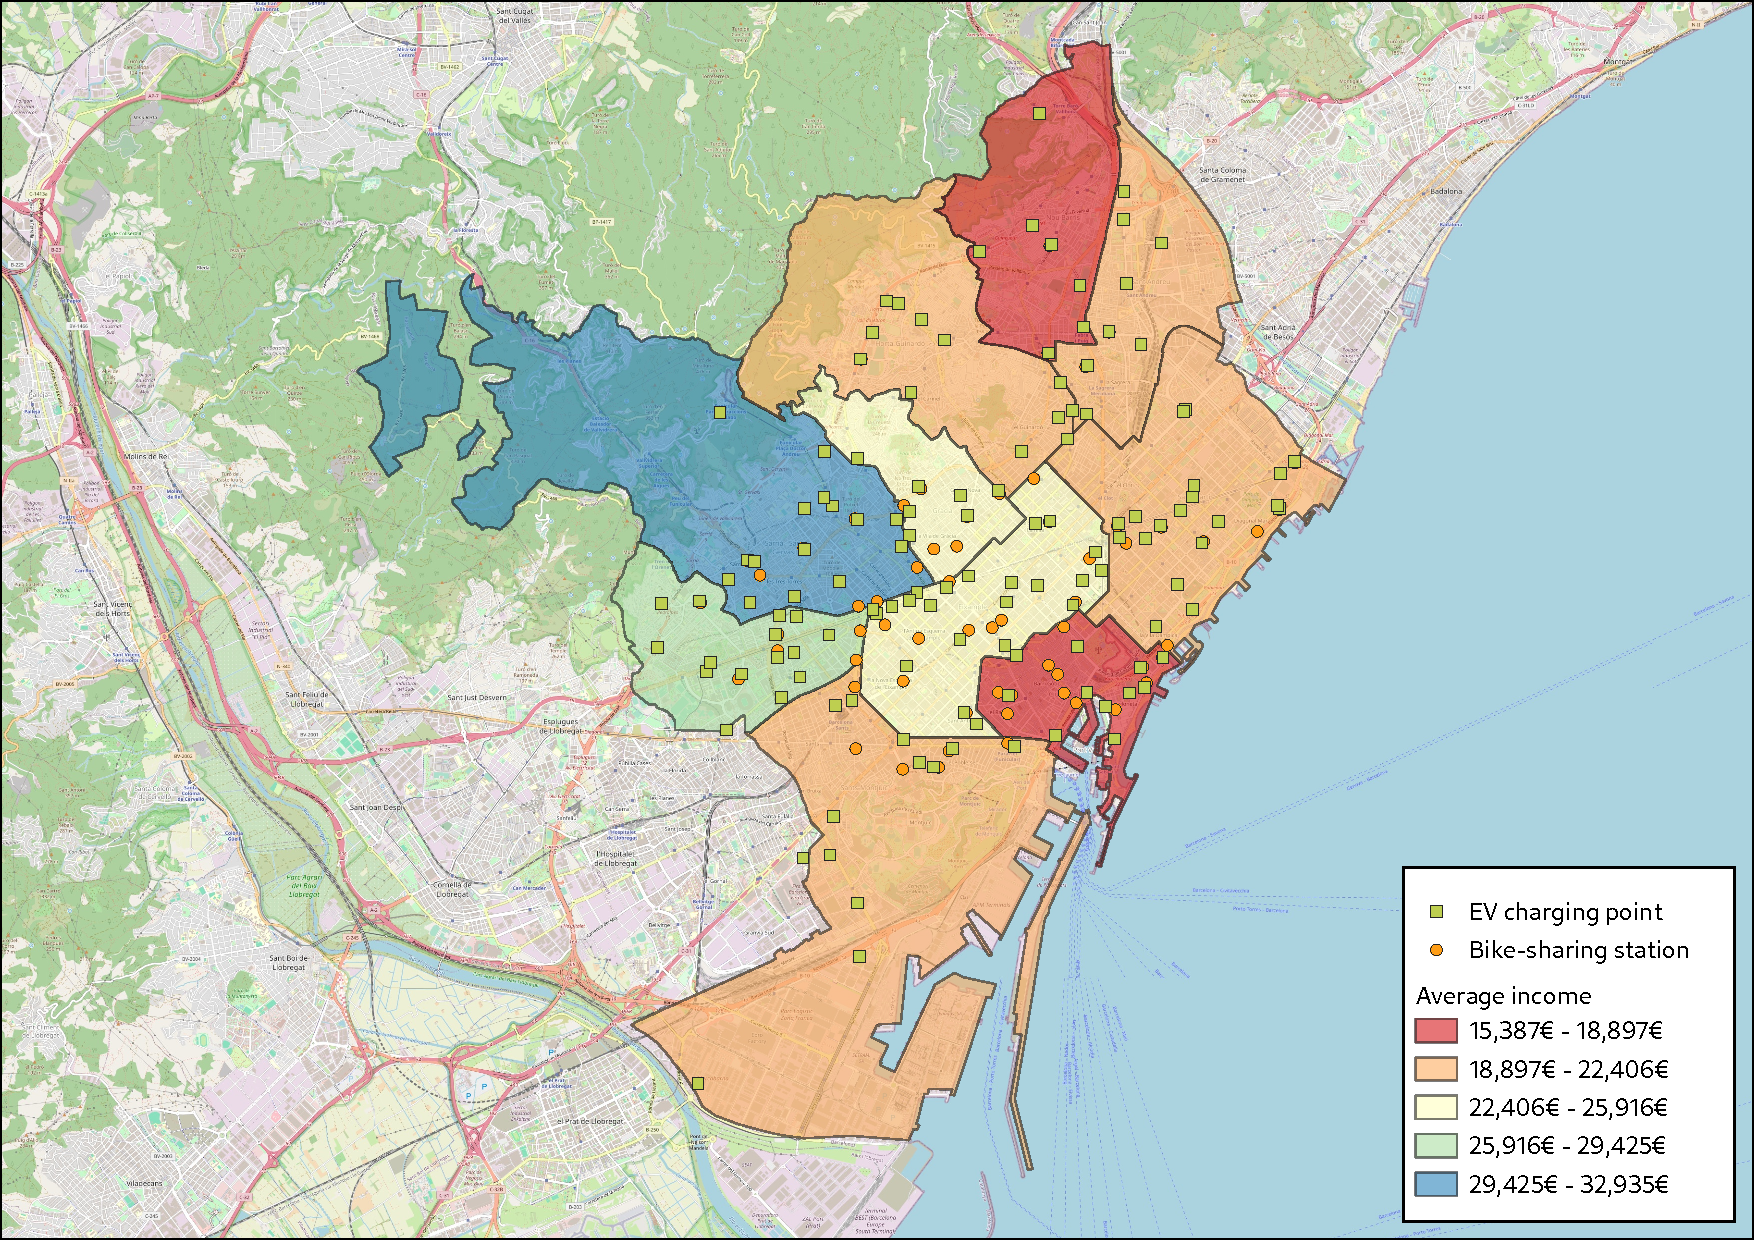
\includegraphics[width=\textwidth]{figures/Barcelona_data.pdf}
    \caption{Assessment of sustainability and equitable distribution of services in Barcelona, focusing on the placement of bike-sharing and electric vehicle charging stations.}
    \label{fig:data_barcelona}
\end{figure}

\begin{figure}[htb]
    \centering
    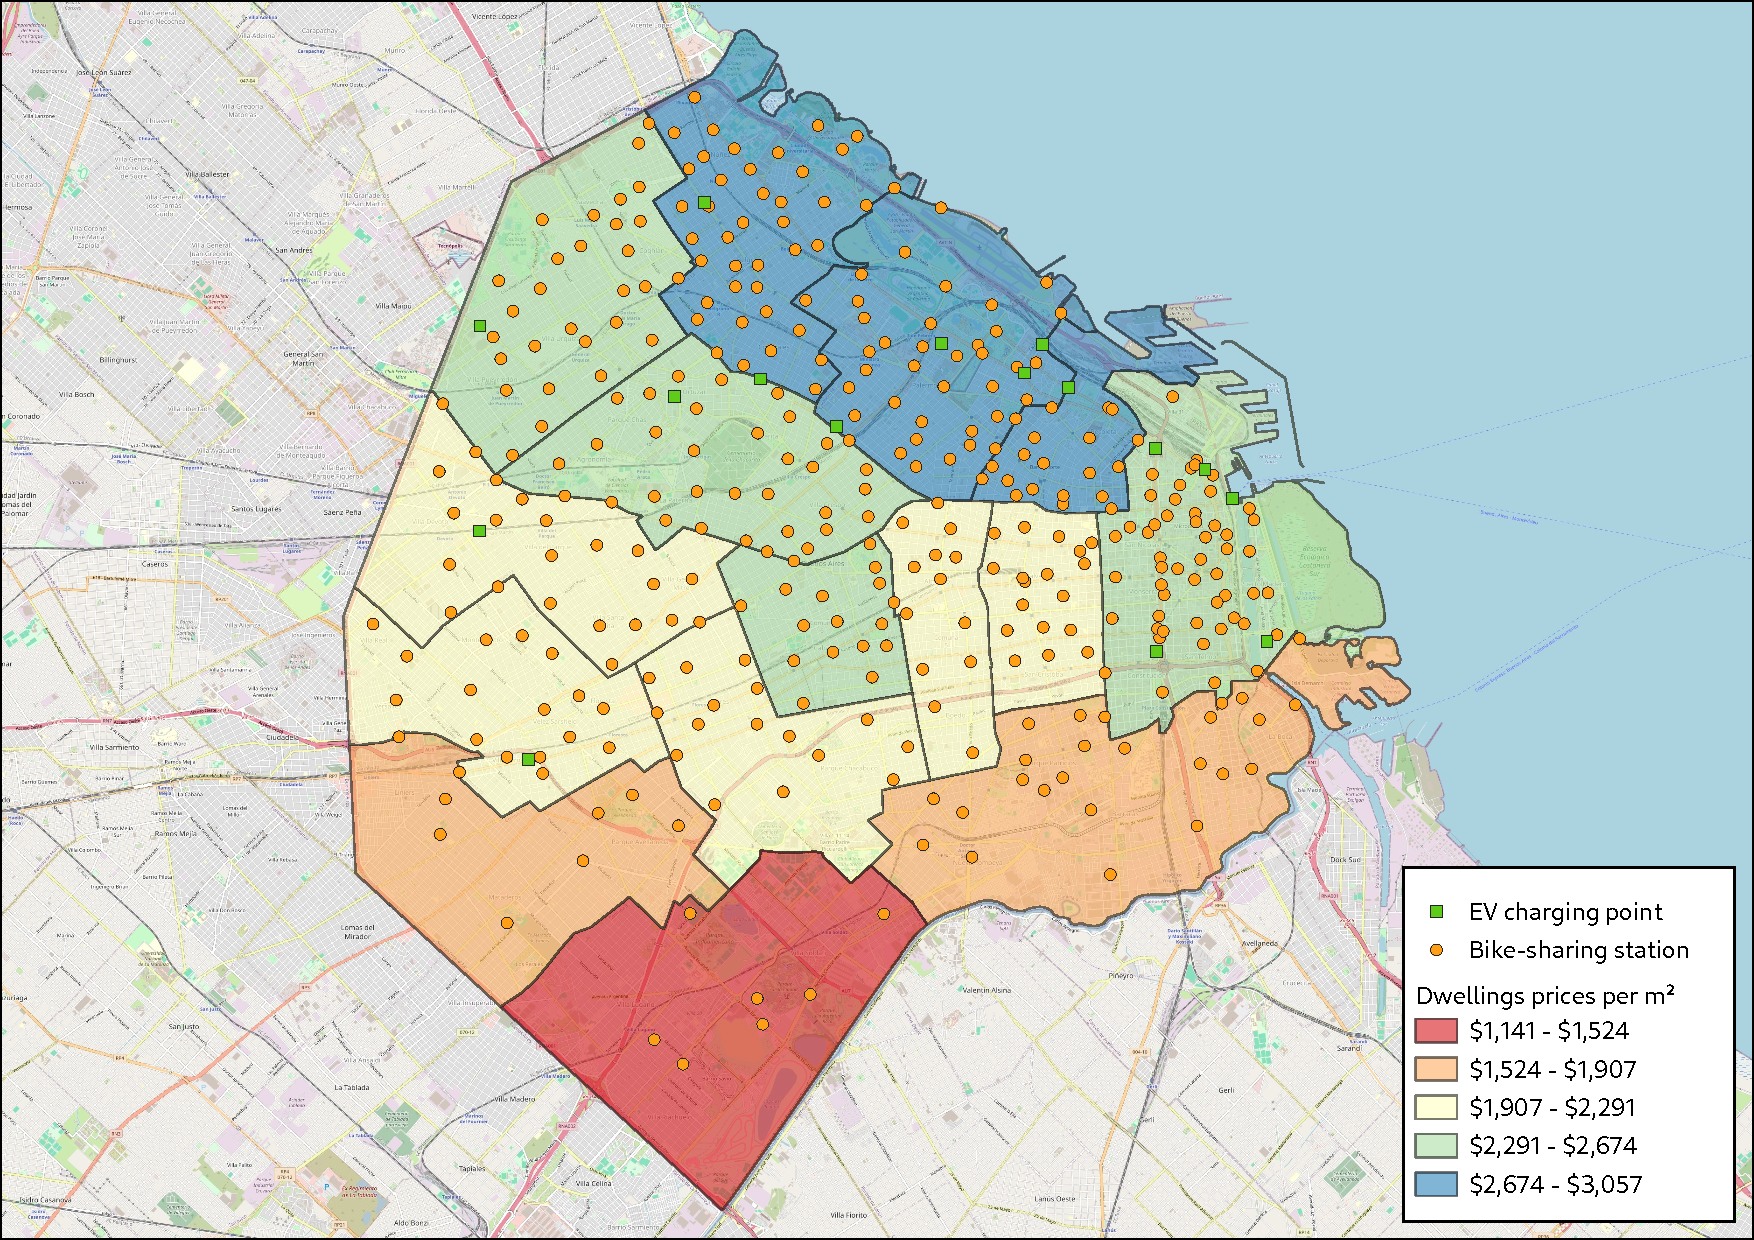
\includegraphics[width=\textwidth]{figures/Buenos_Aires_data.pdf}
    \caption{Assessment of sustainability and equitable distribution of services in Buenos Aires, focusing on the placement of bike-sharing and electric vehicle charging stations.}
    \label{fig:data_buenos_aires}
\end{figure}

The orange dots on the maps represent the locations of bike-sharing stations, while the green squares represent the locations of EV charging points. In both Helsinki and Buenos Aires, the concentration of these services in wealthier areas highlights a significant disparity in the distribution of public services. In Helsinki, this disparity is even more pronounced, with economically disadvantaged areas receiving inadequate access to both bike-sharing locations and EV charging points. Therefore, it can be concluded that the distribution of public services is inadequate, especially concerning bike-sharing. Given that access to bicycles should be universal, it is crucial that less affluent areas are also sufficiently served by these alternative mobility services. In contrast to the uneven distribution seen in Helsinki and Buenos Aires, the distribution of EV charging points in Barcelona is more balanced, with charging stations available throughout most of the city, regardless of residents' income. However, the current distribution of these services in peripheral areas remains insufficient, suggesting that our findings may have significant implications for future urban planning.

Figures~\ref{fig:risk_helsinki}, \ref{fig:risk_barcelona}, and \ref{fig:risk_buenos_aires} illustrate the findings of the resilience assessment conducted using the CityZones tool. Specifically, a comparison was made between the resilience of the cities and the wealth of their citizens across various city zones. In this analysis, red areas indicate lower resilience, while the green ones are considered more resilient. As depicted in Figure~\ref{fig:risk_helsinki}, the prioritization of high-income regions in Helsinki is clear, with the resilience map predominantly displaying green shades around the most expensive neighborhoods. Interestingly, some lower-cost areas in the northern part of the city show a relatively high level of resilience. A similar trend is noted in Barcelona (Figure~\ref{fig:risk_barcelona}), where the most resilient zones correspond to the highest-income neighborhoods, whereas the lowest-income regions exhibit lower resilience. In Buenos Aires (Figure~\ref{fig:risk_buenos_aires}), the city's southern area reveals a pattern of low income and low resilience, except for the costly neighborhoods near the sea, which have a low resilience classification.

\begin{figure}[htb]
    \centering
    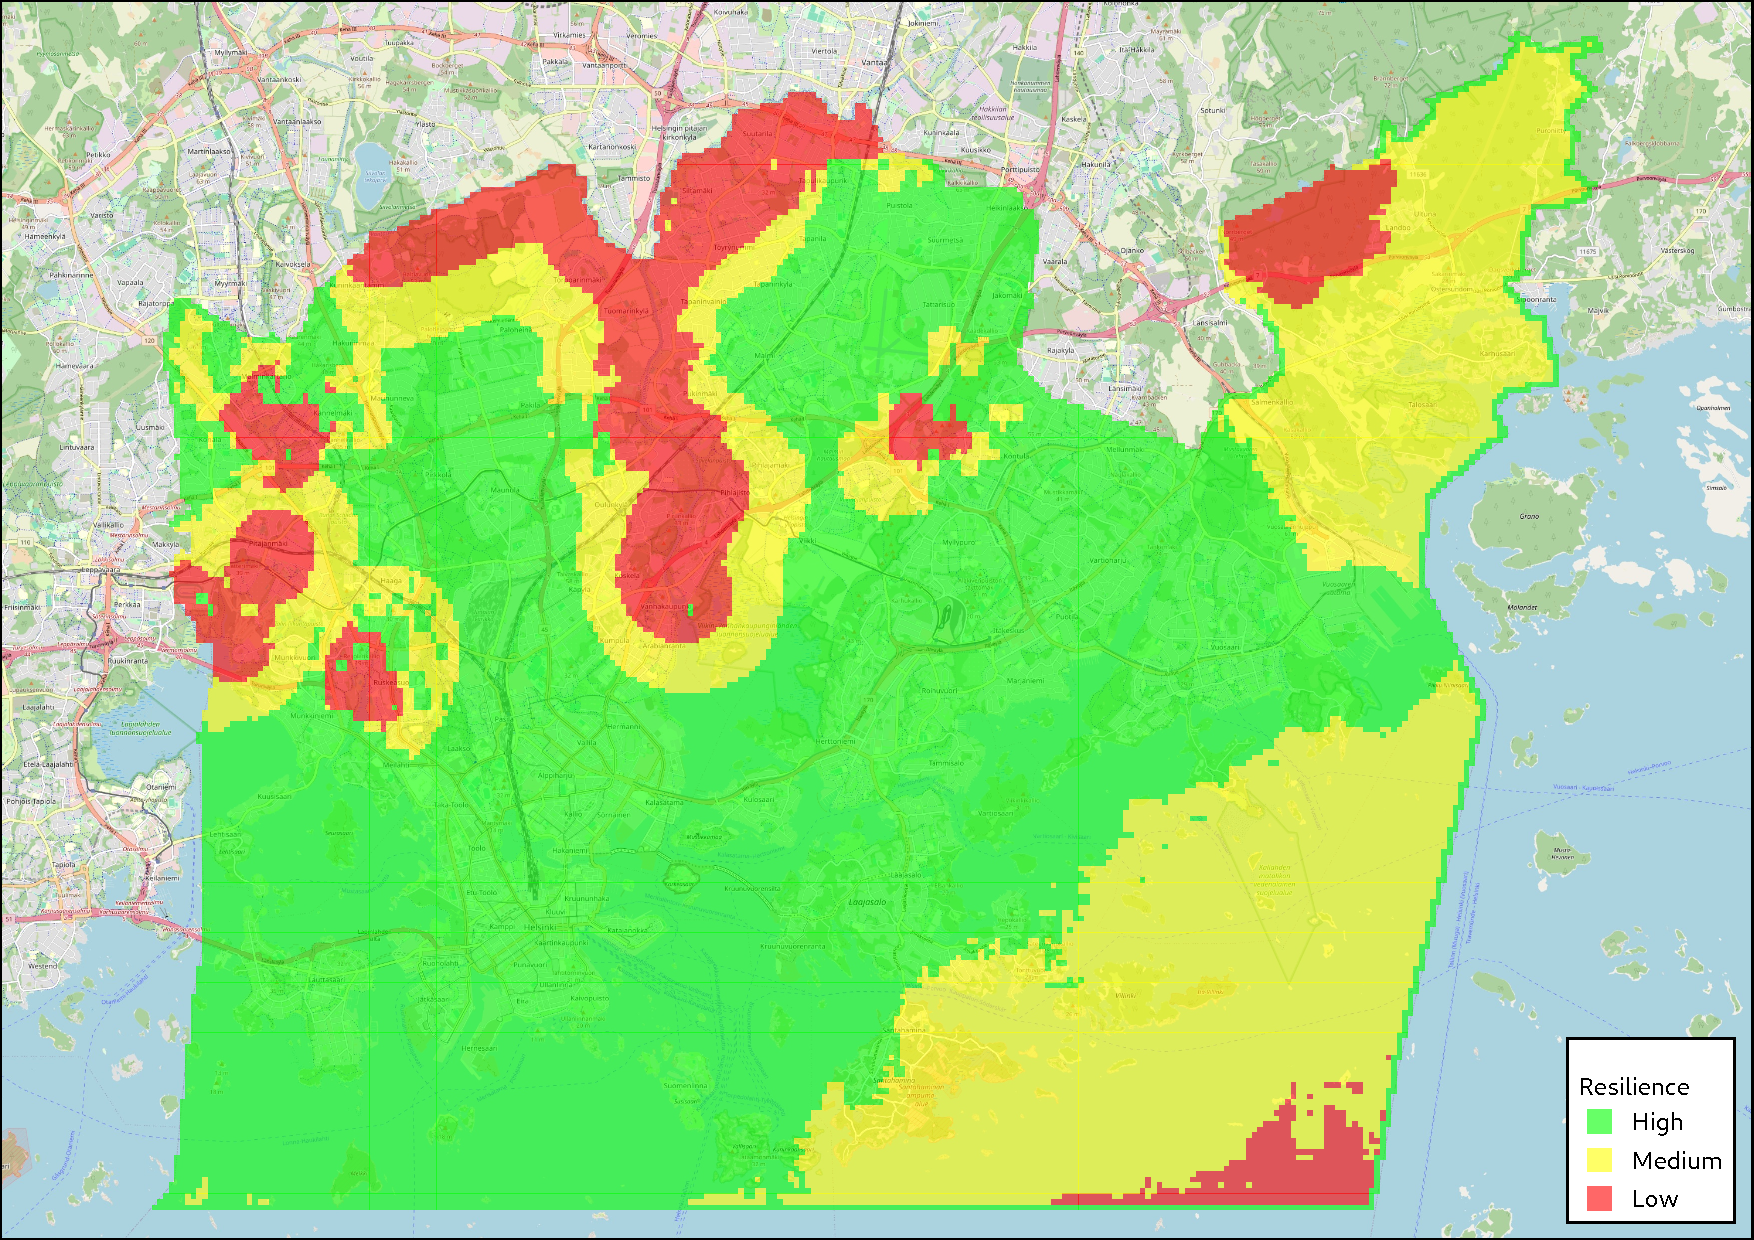
\includegraphics[width=\textwidth]{figures/Helsinki_risk.pdf}
    \caption{A classification of areas within Helsinki based on their resilience to emergencies.}
    \label{fig:risk_helsinki}
\end{figure}

\begin{figure}[htb]
    \centering
    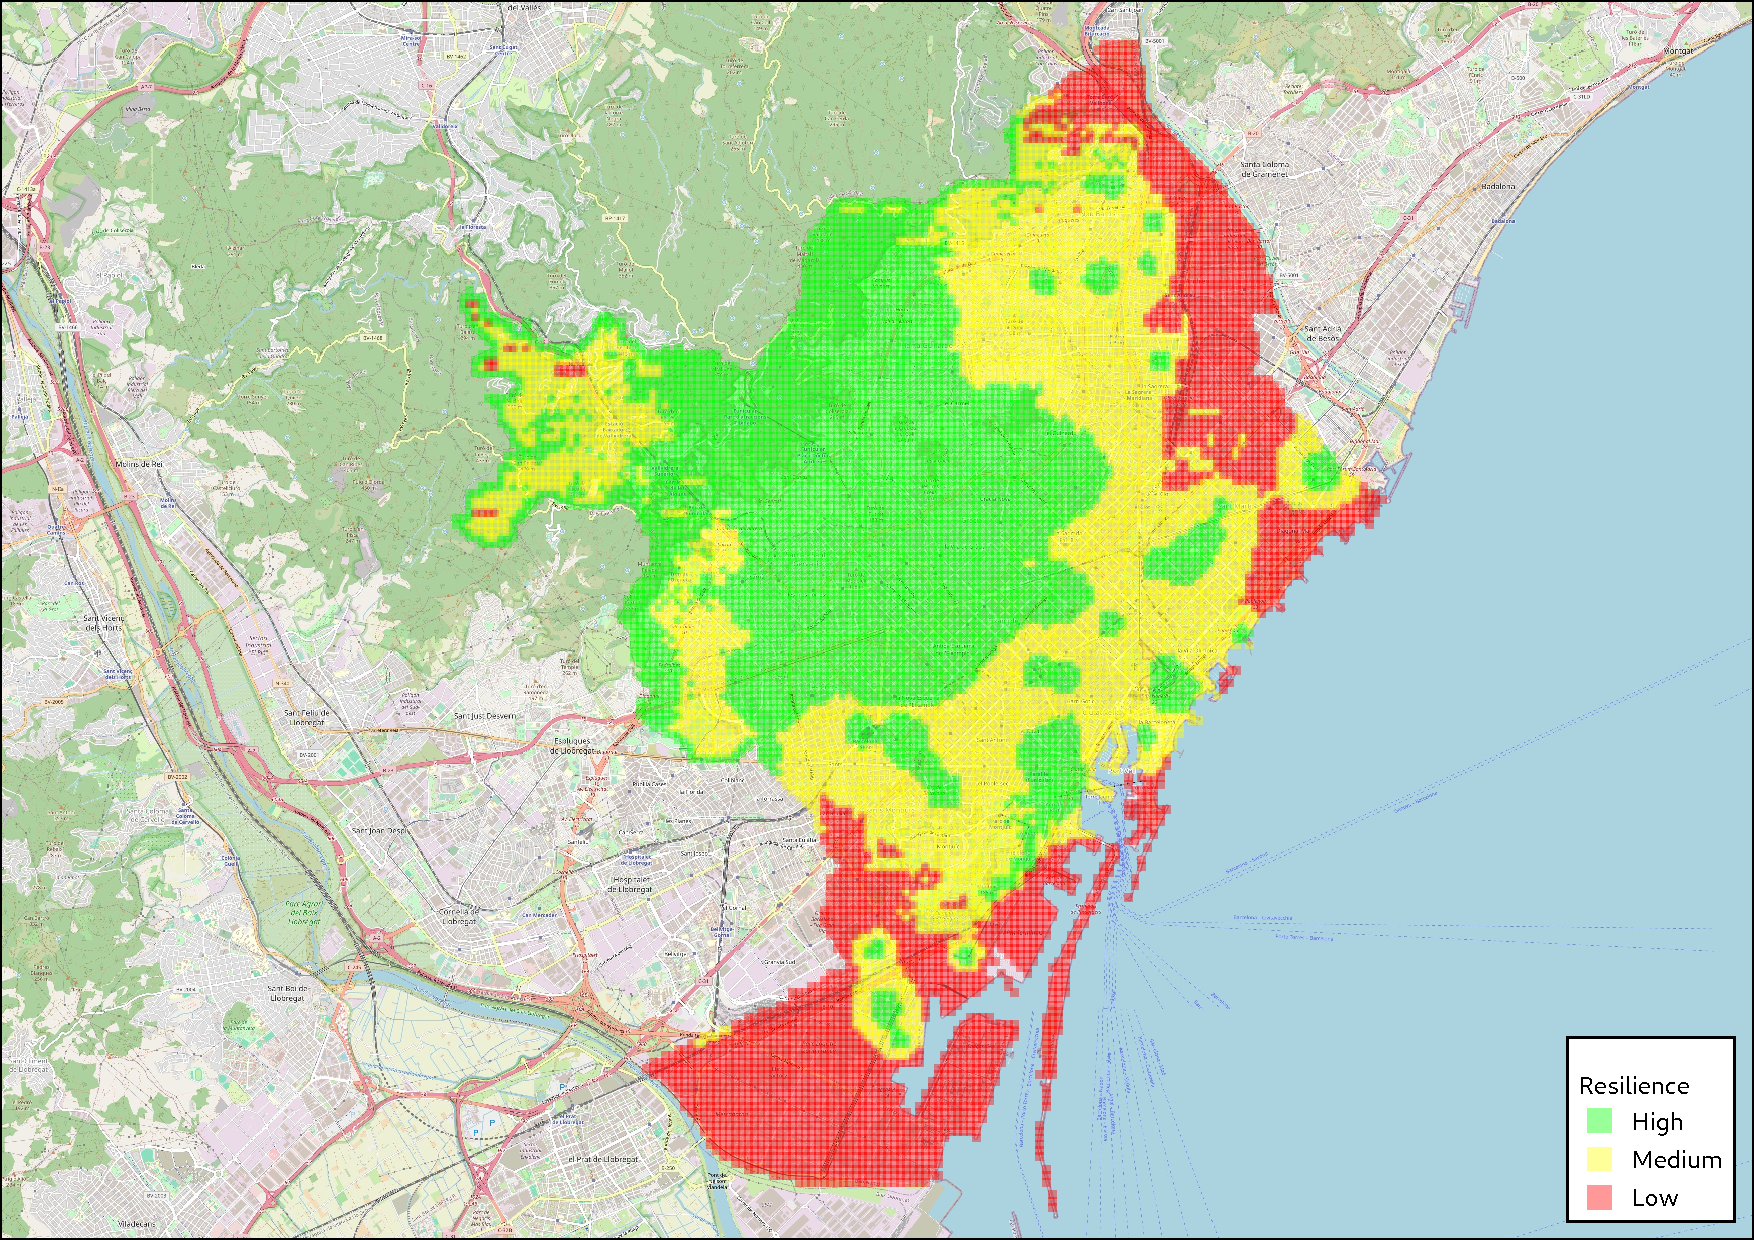
\includegraphics[width=\textwidth]{figures/Barcelona_risk.pdf}
    \caption{A classification of areas within Barcelona based on their resilience to emergencies.}
    \label{fig:risk_barcelona}
\end{figure}

\begin{figure}[htb]
    \centering
    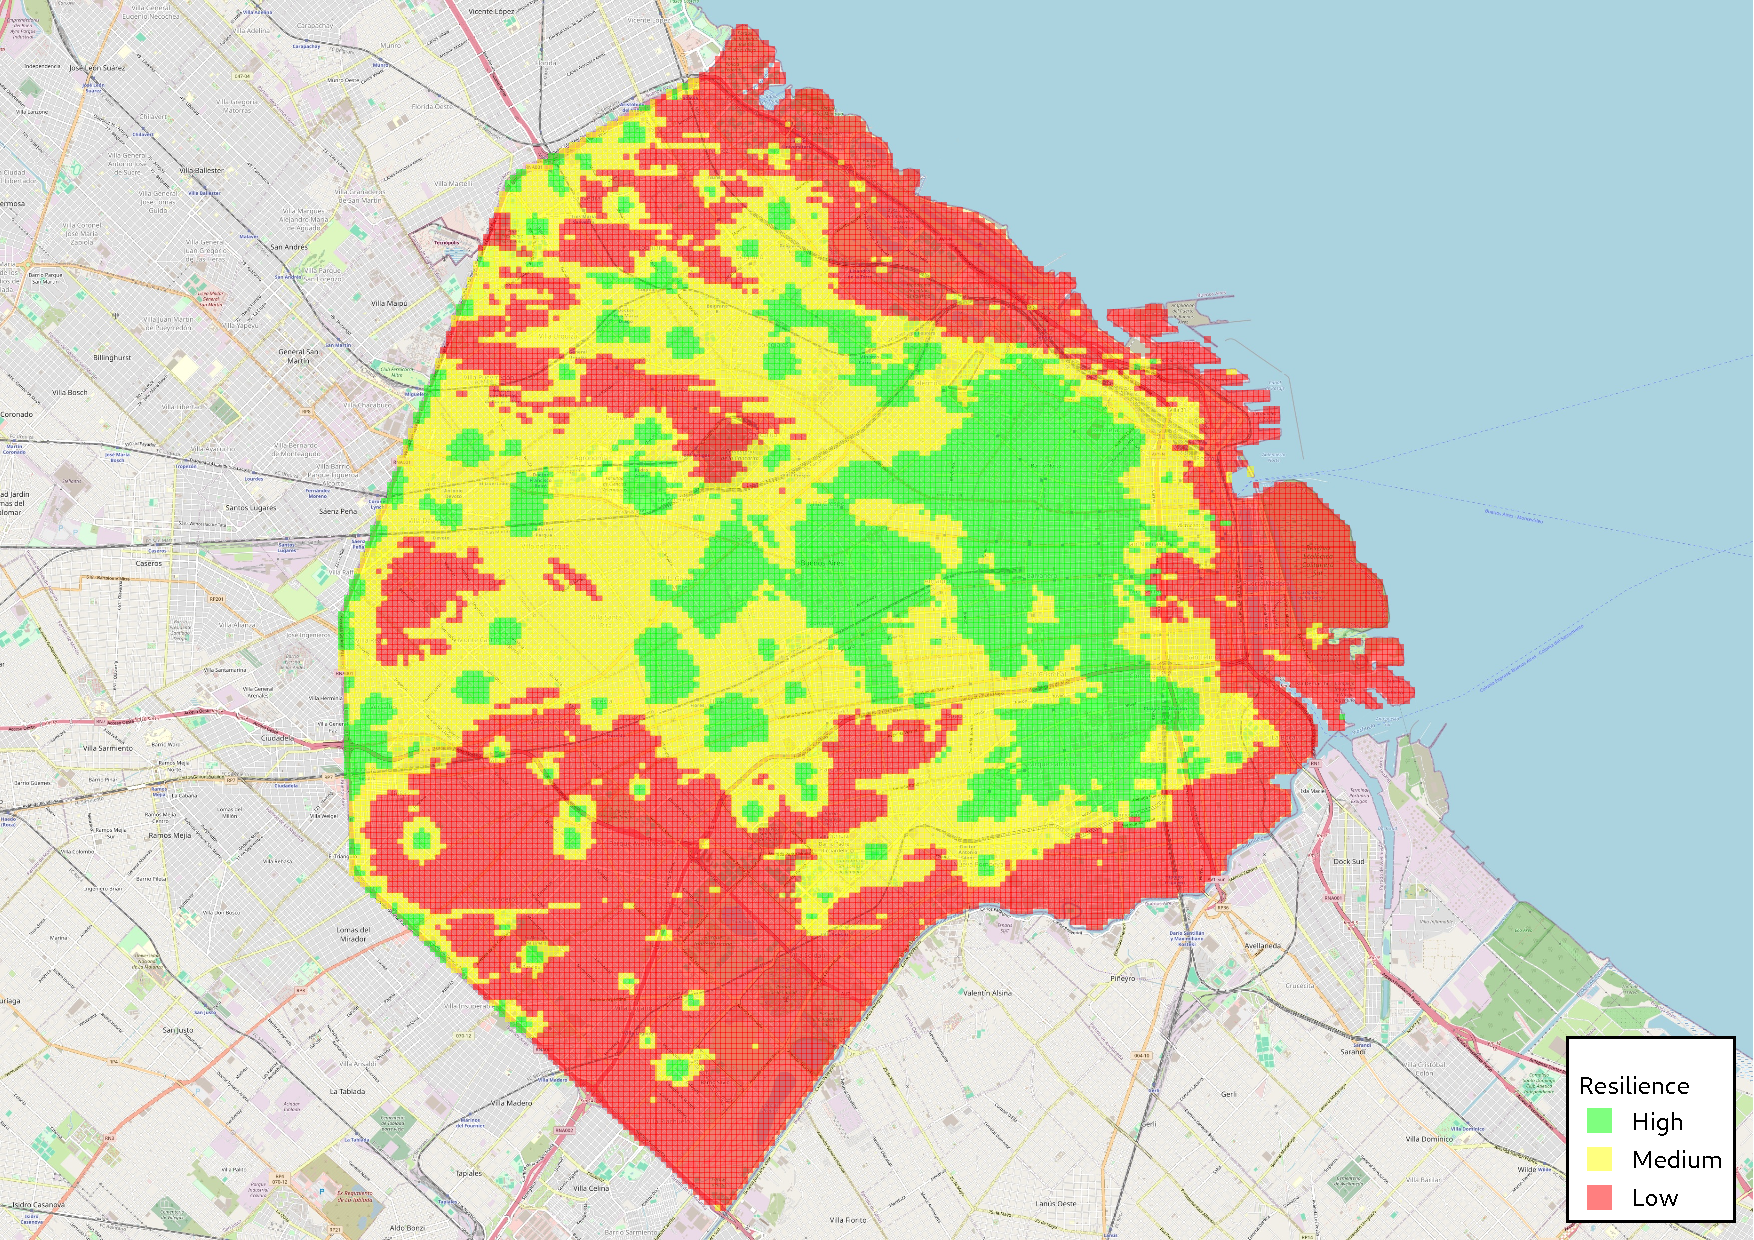
\includegraphics[width=\textwidth]{figures/Buenos_Aires_risk.pdf}
    \caption{A classification of areas within Buenos Aires based on their resilience to emergencies.}
    \label{fig:risk_buenos_aires}
\end{figure}

The open data analysis and resilience assessment indicated that some smart city initiatives fail to address the needs of those who truly require them, exacerbating equity issues in urban areas. For the concept of intelligent cities to develop fully, technology solutions related to city services must improve the well-being of all citizens, encompassing the entire city without socioeconomic prioritization.

%%%%%%%%%%%

\section{Discussion}
\label{sec:discussion}
%[DANIEL]
The current concept of smart cities entails the notion of a ``smart mentality'', as articulated by~\cite{Vanolo2013,Zhang2022}, highlighting how smart city policies introduce new ways of managing cities but also impose a new moral order by defining what constitutes a ``good'' or ``bad'' city based on specific parameters. This underscores the need for a multidimensional perspective that goes beyond the reliance on technology towards influencing. Conversely, intelligent cities adopt a holistic approach, integrating technology efficiency with urban social functions sustained by sustainability, reliability and equity principles. This paradigm encompasses efficient management, improved service delivery based on citizens' real needs and greater resilience to environmental and urban spatial and temporal dynamics. Consequently, a thorough understanding of how intelligent cities might reshape future development requires a comprehensive analysis of the technological and social pillars underpinning our cities.

The findings of the experiments provide tangible evidence that the advancement of technology in smart cities has not been equitably distributed across different socioeconomic groups. The results revealed that economically advantaged areas within cities exhibited a greater prevalence of these services, while those with lower incomes were less well-served. This discrepancy underscores the challenge of implementing intelligent city solutions that benefit all citizens, regardless of their financial status. Furthermore, it became evident that resilience in cities also correlates with wealthier areas being better equipped to handle crises, while low-income zones remain vulnerable. Such an uneven distribution across socioeconomic lines indicates that addressing the digital divide remains a significant challenge for policymakers. 

Although this review provides valuable insights into the integration of smart solutions in urban environments and their impact, it also highlights the significance of open data for urban development. The utilization of publicly accessible datasets, which exhibit varying degrees of detail and consistency across urban contexts, illustrates the potential for enhanced transparency and citizen engagement in the evaluation of urban service efficacy. By relying on open data, the study reinforces the necessity for accessible and comprehensive data to foster more informed decision-making processes. Consequently, open data can be a potential enabler to drive innovation in intelligent city planning and hold cities accountable for ensuring that enhancements contribute to sustainability while retaining resilience and are distributed equitably. 

Furthermore, despite the evaluation focusing on three specific cities, the findings are likely to reflect broader trends applicable to many urban areas, irrespective of their level of technological advancement or socioeconomic status. It should be noted, however, that the present study does not propose the uniform deployment of \textit{all} services across the entire city. The objective of intelligent cities is not to guarantee absolute smart service coverage but rather to prioritize the requirements of specific areas based on their existing infrastructure and specific needs. For example, the investment in bike-sharing programs may be less necessary in zones already well-served by an extensive and efficient transportation system, such as trains, buses, or metros. Instead, resources could be allocated to areas lacking alternative transportation modes. Despite this, the results from our study did not provide evidence of such a strategic, needs-based urban deployment. The absence of clear planning strategies that align services with actual city requirements highlights a gap in current smart city implementations.

The following subsections build on these insights to provide a more detailed examination of intelligent city implementation. Through an analysis of how social domains can be effectively integrated into the dimensions of smart urban services, we present a comprehensive theoretical framework that can guide the creation of truly transformative urban environments. This discussion also identifies critical areas for future research, outlining potential pathways to advance the development of intelligent cities and enhance their societal impact.

\subsection{Implementing intelligent cities} 

The alignment of urban technologies with the fundamental urban social domain highlights the broader ambition of intelligent cities to address complex societal needs. This approach would represent a shift from traditional smart cities, which often focus on optimizing individual systems~\cite{javedFutureSmartCities2022,ketuContemporarySurveyIoT2022}, to intelligent cities that prioritize the entire citizen-centered urban ecosystem. Intelligent cities strive to improve operational efficiencies and foster inclusive and sustainable communities by carefully embedding technological solutions within the fabric of daily urban life. This comprehensive integration is justified by the growing need for cities to be more than just technologically advanced, considering they must also be socially equitable and resilient \cite{samarakkodyResilientSmartCities2022,toliInequalitySustainabilitySmartCity2020}. 

Implementing smart cities involves considering various social, economic, technical, and infrastructural aspects that must be carefully addressed to realize their full potential. One of the primary objectives is the integration of diverse technologies and systems into a cohesive urban digital infrastructure. This synergy requires robust interoperability standards to ensure that various technologies can effectively communicate and function together. Additionally, the vast amounts of data generated by intelligent cities necessitate substantial investments in data storage, processing, and cybersecurity infrastructure to manage and protect sensitive information. Implementing intelligent cities also requires a strategic approach to upgrading existing urban infrastructure to seamlessly accommodate new technologies, carefully planning to address the costs and logistical complexities, particularly in older cities with legacy systems.

Building on the strategic need to update existing urban infrastructure, ensuring scalability is key to successfully implementing intelligent cities. Technologies that perform well in smaller-scale pilot projects must be carefully adapted to function across an entire urban environment, considering the socioeconomic realities and, most importantly, the citizens' priorities. This highlights the need for long-term projects designed with adaptive and flexible infrastructure that can evolve alongside technological advancements while adjusting to urban needs.
However, achieving this vision requires a coordinated effort from the public and private sectors, with strategic planning and investment to build resilient and future-ready urban environments.

Despite the recent efforts, the social divide remains a significant concern since access to enhanced urban services is often uneven, disproportionately benefiting areas with higher socioeconomic status. To counter this, an intelligent city must focus on infrastructure and services without distinctions, promoting sustainability and contributing to avoiding inequalities. Promoting sustainability while addressing inequality should be central to all urban planning initiatives. In this sense, implementing solutions that ensure all areas of a city benefit from enhanced urban services is a fundamental goal that must be embraced by all stakeholders involved in urban development. To this end, research innovation and industry solutions must focus on accessibility and equity in technology deployment. This means policies and initiatives must be in place to ensure that urban systems leave no one behind.

It is also important to remark that irrespective of their level of `smartness', cities will always be dynamic entities that evolve spatially and temporally, shaped by complex interactions between humans and their environment. Although concepts such as urban metabolism~\cite{KavitiMusango2020} frequently characterize cities as self-sustaining entities, we acknowledge that these are human-made constructs. The true essence of a city is revealed through its dynamic fluxes, which manifest in the form of resource consumption, waste production and human habitation. These tangible elements represent the city as a ``living organism'' driven by human activity. Therefore, a city is thus inextricably linked with patterns within its physical structure (spatial domain) and its dynamic evolution over time (temporal domain). Therefore, these spatiotemporal dynamics must be fully understood if effective strategies for urban development that prioritize human domains and address the challenges posed by urbanization are to be developed.

Understanding a city's spatiotemporal dynamics is essential for capturing the complexities of urban flow and developing digital infrastructure tailored to societal needs~\cite{bittencourtDatadrivenClusteringApproach2024}. However, realizing this potential requires significant advancements since current urban capabilities often fall short of the demands for such a holistic understanding. Addressing these challenges necessitates a bottom-up approach that integrates infrastructure development, which remains one of the most formidable long-term goals for urban planners.

Such a bottom-up perspective focuses on leveraging IoT devices to gather geolocated data at a granular level, encompassing urban parameters in real-time, such as traffic patterns, air quality, energy usage, and public safety. The myriad of data these devices collect requires robust distributed computing frameworks. Geospatial analytics powered by machine learning algorithms can thus uncover patterns and trends that might go unnoticed. Furthermore, these data-driven approaches could be integrated with dynamic visualization tools so that city planners and policymakers can achieve a comprehensive understanding of urban dynamics in real-time. Finally, decision-making policies can be more adaptive and responsive to these insights, ensuring that urban services are optimized to meet the cities' needs. Despite ongoing research in this area, there are still opportunities for innovation that will empower our cities.

\subsection{Perspectives and future works}

The evolution of intelligent cities represents a significant shift in the interaction between technology and urban life. This is evidenced by the transformation of urban infrastructures and the reshaping of societal norms, behaviors, and institutions. As these systems evolve, they can engage in a continuous, dynamic adaptation process, driving a technological transition that makes cities more sustainable, resilient, and human-centered. Our vision of intelligent cities allows us to identify several key areas for future research and innovation, as well as gaps in the development of cities worldwide. 

\begin{itemize}
    \item \textbf{Urban interoperability:} As urban areas become increasingly reliant on data-driven decision-making and technological integration, future research should prioritize the development of robust frameworks for interoperability and integration across diverse urban systems. This entails the establishment of standardized protocols for data exchange and system interaction, which will prove instrumental in surmounting the current infrastructural and technical challenges.  
    
    \item \textbf{Technological scalability:} Further investigation is required into the potential of technologies that have demonstrated effectiveness in small-scale deployments, such as cities' pilot projects, living labs or research simulations, to be effectively and efficiently deployed in larger, more complex urban environments, while ensuring equity.
    
    \item \textbf{Digital divide:} Ensuring equitable access is another critical area of future research. This involves studying and developing affordable technologies adopting inclusive design principles and policies.

    \item \textbf{Understand city dynamic needs:} Researchers should focus on advancing geospatial analytics and machine learning techniques to predict and manage urban flows. This includes embedding city information into real-time visualization and predictive platforms tailored to urban planners and policymakers. 

    \item \textbf{Emerging technologies:} Studying the impact of emerging technologies such as 5G, edge computing, and blockchain on urban management could offer new insights into creating resilient and adaptive city infrastructures. Furthermore, research on the use of Cyber-Physical–Social Systems would facilitate the integration of the technological and social domains within a system-of-systems framework.

    \item \textbf{Interdisciplinary research:} To create a more holistic understanding of intelligent cities, we need studies that integrate social sciences, urban planning, and technology development. Such research should explore the sociotechnical implications, including ethical considerations around privacy and surveillance and developing transparent, inclusive, and adaptable governance models.
\end{itemize}


\section{Conclusions}
\label{sec:conclusion}

The concept of Intelligent Cities represents a significant transition from conventional technology-centric approaches to urban planning, which has been the dominant paradigm in the field for several decades, to a more holistic and human-centered methodology. In contrast to the prevailing trend of developing smart cities, which is primarily concerned with operational efficiencies and technological innovation, intelligent cities will seek to integrate technologies with the essential social functions that shape urban life. Doing so, this new reasoning will emphasize sustainability, resilience, and equity as fundamental urban development principles, ensuring cities advance technologically aligned with their population's diverse needs.

This article examined the complex and varied aspects of intelligent cities, focusing on the difficulties of incorporating sophisticated technologies into the urban environment. The analysis of the social and technical challenges associated with the implementation of extensive urban digital infrastructures underscored the necessity for scalable, adaptable, and inclusive technologies. Through a comprehensive literature review and data-driven assessments of some current smart cities, we emphasized the importance of design approaches in which the needs of citizens and the dynamics of urban development will support the creation of truly intelligent infrastructures. 

The necessity of ensuring equitable access to urban services and technologies is of paramount importance. Therefore, we believe that the success of intelligent cities will depend on their capacity to align technological developments with human well-being. By prioritizing citizen-centric urban services, cities will be able to establish a model for creating urban environments that are not only technologically advanced but also equitable, sustainable and resilient. 

%%%%%%%%%%%%%%%%%%%%%%%%%%%%%%%%%%%%%%%%%%
\vspace{6pt} 

%%%%%%%%%%%%%%%%%%%%%%%%%%%%%%%%%%%%%%%%%%

%% optional
%\supplementary{The following supporting information can be downloaded at:  \linksupplementary{s1}, Figure S1: title; Table S1: title; Video S1: title.}

% Only for journal Methods and Protocols:
% If you wish to submit a video article, please do so with any other supplementary material.
% \supplementary{The following supporting information can be downloaded at: \linksupplementary{s1}, Figure S1: title; Table S1: title; Video S1: title. A supporting video article is available at doi: link.}

% Only used for preprtints:
% \supplementary{The following supporting information can be downloaded at the website of this paper posted on \href{https://www.preprints.org/}{Preprints.org}.}

% Only for journal Hardware:
% If you wish to submit a video article, please do so with any other supplementary material.
% \supplementary{The following supporting information can be downloaded at: \linksupplementary{s1}, Figure S1: title; Table S1: title; Video S1: title.\vspace{6pt}\\
%\begin{tabularx}{\textwidth}{lll}
%\toprule
%\textbf{Name} & \textbf{Type} & \textbf{Description} \\
%\midrule
%S1 & Python script (.py) & Script of python source code used in XX \\
%S2 & Text (.txt) & Script of modelling code used to make Figure X \\
%S3 & Text (.txt) & Raw data from experiment X \\
%S4 & Video (.mp4) & Video demonstrating the hardware in use \\
%... & ... & ... \\
%\bottomrule
%\end{tabularx}
%}

%%%%%%%%%%%%%%%%%%%%%%%%%%%%%%%%%%%%%%%%%%
\authorcontributions{Conceptualization, J.C.N.B., T.C.J., J.P.J.P, and D.G.C.; methodology, J.C.N.B., D.G.C.; formal analysis, D.G.C., J.C.N.B., J.P.J.P, and T.C.J.; data curation, J.C.N.B., D.G.C., and J.P.J.P;  writing---original draft preparation, J.C.N.B., D.G.C., T.C.J., and J.P.J.P; writing---review and editing, D.G.C.; supervision, D.G.C.; All authors have read and agreed to the published version of the manuscript.}


\funding{This research was supported by the Associate Laboratory Advanced Production and Intelligent Systems – ARISE LA/P/0112/2020 (DOI 10.54499/LA/P/0112/2020), by the Base Funding (UIDB/00147/2020) and Programmatic Funding (UIDP/00147/2020) of the R\&D Unit Center for Systems and Technologies -- SYSTEC, and by the Fundação para a Ciência e a Tecnologia (FCT) through the PhD scholarship (2024.02446.BD).}

% \institutionalreview{In this section, you should add the Institutional Review Board Statement and approval number, if relevant to your study. You might choose to exclude this statement if the study did not require ethical approval. Please note that the Editorial Office might ask you for further information. Please add “The study was conducted in accordance with the Declaration of Helsinki, and approved by the Institutional Review Board (or Ethics Committee) of NAME OF INSTITUTE (protocol code XXX and date of approval).” for studies involving humans. OR “The animal study protocol was approved by the Institutional Review Board (or Ethics Committee) of NAME OF INSTITUTE (protocol code XXX and date of approval).” for studies involving animals. OR “Ethical review and approval were waived for this study due to REASON (please provide a detailed justification).” OR “Not applicable” for studies not involving humans or animals.}

% \informedconsent{Any research article describing a study involving humans should contain this statement. Please add ``Informed consent was obtained from all subjects involved in the study.'' OR ``Patient consent was waived due to REASON (please provide a detailed justification).'' OR ``Not applicable'' for studies not involving humans. You might also choose to exclude this statement if the study did not involve humans.

% Written informed consent for publication must be obtained from participating patients who can be identified (including by the patients themselves). Please state ``Written informed consent has been obtained from the patient(s) to publish this paper'' if applicable.}

\dataavailability{Dataset available on request from the authors.} 

% Only for journal Drones
%\durcstatement{Current research is limited to the [please insert a specific academic field, e.g., XXX], which is beneficial [share benefits and/or primary use] and does not pose a threat to public health or national security. Authors acknowledge the dual-use potential of the research involving xxx and confirm that all necessary precautions have been taken to prevent potential misuse. As an ethical responsibility, authors strictly adhere to relevant national and international laws about DURC. Authors advocate for responsible deployment, ethical considerations, regulatory compliance, and transparent reporting to mitigate misuse risks and foster beneficial outcomes.}

% Only for journal Nursing Reports
%\publicinvolvement{Please describe how the public (patients, consumers, carers) were involved in the research. Consider reporting against the GRIPP2 (Guidance for Reporting Involvement of Patients and the Public) checklist. If the public were not involved in any aspect of the research add: ``No public involvement in any aspect of this research''.}
%
%% Only for journal Nursing Reports
%\guidelinesstandards{Please add a statement indicating which reporting guideline was used when drafting the report. For example, ``This manuscript was drafted against the XXX (the full name of reporting guidelines and citation) for XXX (type of research) research''. A complete list of reporting guidelines can be accessed via the equator network: \url{https://www.equator-network.org/}.}
%
%% Only for journal Nursing Reports
%\useofartificialintelligence{Please describe in detail any and all uses of artificial intelligence (AI) or AI-assisted tools used in the preparation of the manuscript. This may include, but is not limited to, language translation, language editing and grammar, or generating text. Alternatively, please state that “AI or AI-assisted tools were not used in drafting any aspect of this manuscript”.}

% \acknowledgments{In this section you can acknowledge any support given which is not covered by the author contribution or funding sections. This may include administrative and technical support, or donations in kind (e.g., materials used for experiments).}

\conflictsofinterest{The authors declare no conflict of interest.} 

%%%%%%%%%%%%%%%%%%%%%%%%%%%%%%%%%%%%%%%%%%
%% Optional

%% Only for journal Encyclopedia
%\entrylink{The Link to this entry published on the encyclopedia platform.}


%\section[\appendixname~\thesection]{}
%All appendix sections must be cited in the main text. In the appendices, Figures, Tables, etc. should be labeled, starting with ``A''---e.g., Figure A1, Figure A2, etc.

%%%%%%%%%%%%%%%%%%%%%%%%%%%%%%%%%%%%%%%%%%
%\isPreprints{}{% This command is only used for ``preprints''.
%\begin{adjustwidth}{-\extralength}{0cm}
%} % If the paper is ``preprints'', please uncomment this parenthesis.
%\printendnotes[custom] % Un-comment to print a list of endnotes

\reftitle{References}

% Please provide either the correct journal abbreviation (e.g. according to the “List of Title Word Abbreviations” http://www.issn.org/services/online-services/access-to-the-ltwa/) or the full name of the journal.
% Citations and References in Supplementary files are permitted provided that they also appear in the reference list here. 

%=====================================
% References, variant A: external bibliography
%=====================================
\bibliography{references}

%=====================================
% References, variant B: internal bibliography
%=====================================

% If authors have biography, please use the format below
%\section*{Short Biography of Authors}
%\bio
%{\raisebox{-0.35cm}{
\includegraphics[width=3.5cm,height=5.3cm,clip,keepaspectratio]{Definitions/author1.pdf}}}
%{\textbf{Firstname Lastname} Biography of first author}
%
%\bio
%{\raisebox{-0.35cm}{
\includegraphics[width=3.5cm,height=5.3cm,clip,keepaspectratio]{Definitions/author2.jpg}}}
%{\textbf{Firstname Lastname} Biography of second author}

% For the MDPI journals use author-date citation, please follow the formatting guidelines on http://www.mdpi.com/authors/references
% To cite two works by the same author: \citeauthor{ref-journal-1a} (\citeyear{ref-journal-1a}, \citeyear{ref-journal-1b}). This produces: Whittaker (1967, 1975)
% To cite two works by the same author with specific pages: \citeauthor{ref-journal-3a} (\citeyear{ref-journal-3a}, p. 328; \citeyear{ref-journal-3b}, p.475). This produces: Wong (1999, p. 328; 2000, p. 475)

%%%%%%%%%%%%%%%%%%%%%%%%%%%%%%%%%%%%%%%%%%
%% for journal Sci
%\reviewreports{\\
%Reviewer 1 comments and authors’ response\\
%Reviewer 2 comments and authors’ response\\
%Reviewer 3 comments and authors’ response
%}
%%%%%%%%%%%%%%%%%%%%%%%%%%%%%%%%%%%%%%%%%%
%\PublishersNote{}
%\isPreprints{}{% This command is only used for ``preprints''.
%\end{adjustwidth}
%} % If the paper is ``preprints'', please uncomment this parenthesis.
\end{document}

